\chapter{Release 1:Authentification et gestion des utilisateurs} 
 \minitoc
 \newpage
 \counterwithin{figure}{chapter}
\section{Introduction}
La première release de notre plateforme repose sur la mise en place de fonctionnalités fondamentales, notamment l’authentification et la gestion des utilisateurs, réalisées à travers deux sprints stratégiques.
Ce chapitre décrit de manière structurée le processus de développement adopté, en s’appuyant sur les backlogs ainsi que sur les user stories qui ont guidé la conception et l’implémentation.
Pour chaque sprint, une analyse des cas d’utilisation est présentée, suivie d’une phase de conception illustrée par des diagrammes de séquence, puis d’une phase de réalisation mettant en évidence les interfaces développées.
La section \ref{sec:sprint1-authentification} est consacrée à la sécurisation de l’accès à la plateforme, tandis que la section \ref{sec:sprint2-gestion-utilisateurs} traite de la gestion des utilisateurs et des rôles. Ces deux sprints constituent une base essentielle pour les fonctionnalités analytiques futures.

  \section{Sprint 1: «Authentification»}
  \label{sec:sprint1-authentification}
  Cette section présente les résultats du premier sprint, dédié au développement du module d’authentification de la plateforme. Au cours de ce sprint, les efforts ont été orientés vers la mise en place des fonctionnalités essentielles, notamment l’inscription, la connexion des utilisateurs ainsi que la récupération des mots de passe, tout en intégrant des mécanismes de sécurité basés sur l’authentification et l’autorisation.
  \subsection{Le backlog du sprint 1}
  Dans cette partie, nous présentons le backlog du sprint 1, qui a été élaboré à partir des besoins fonctionnels identifiés pour la fonctionnalité d’authentification. Ce backlog comprend les user stories détaillées, permettant de planifier et de prioriser les tâches à réaliser pendant ce sprint comme le montre le tableau \ref{tab:sprint1_backlog}.
  \begin{table}[H]
\centering
\caption{Backlog du Sprint 1 : Authentification}
\label{tab:sprint1_backlog}
\begin{tabular}{|c|p{4cm}|p{10cm}|c|}
\hline
\textbf{ID} & \textbf{Fonctionnalité} & \textbf{User Story} & \textbf{Priorité} \\
\hline
\multirow{3}{*}{1} & \multirow{3}{*}{Login / S'inscrire} 
& En tant qu’utilisateur, je veux me connecter de manière sécurisée pour accéder à mon espace selon mon rôle. & M \\
\cline{3-4}
& & En tant qu’étudiant, je veux pouvoir créer un compte sur la plateforme afin que mon accès soit validé par l’administrateur. & M \\
\cline{3-4}
& & En tant qu’utilisateur, je veux pouvoir réinitialiser mon mot de passe oublié afin de retrouver l’accès à mon espace personnel. & M\\
\hline
\end{tabular}
\end{table}
 
  \subsection{Analyse}
  Dans cette section, nous proposons une analyse synthétique des cas d’utilisation élaborés durant ce sprint. Chaque cas a été ajusté afin de satisfaire les exigences liées à la gestion de l’authentification au sein de la plateforme.

  \noindent\textbf{Amélioration du cas d’utilisation « inscription »:} 
  
  \noindent L’inscription représente la première étape pour les apprenants souhaitant accéder à la plateforme. En effet, contrairement aux autres acteurs dont les comptes sont créés par l’administrateur, seuls les apprenants passent par cette étape. La figure \ref{fig:usecase} illustre le comportement dynamique de ce processus à travers un diagramme de cas d’utilisation.
  \begin{figure}[H]
    \centering
    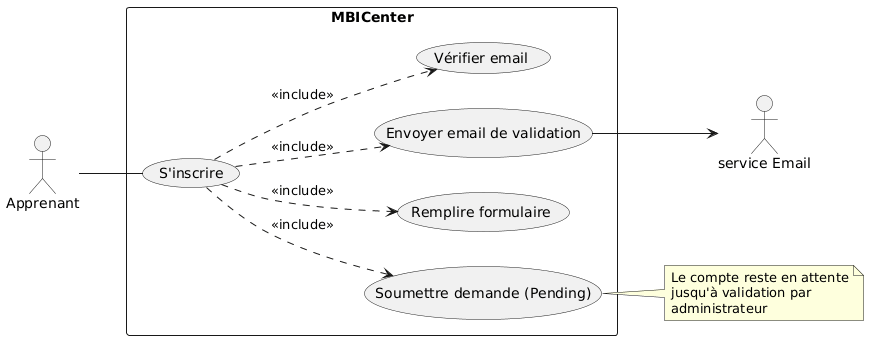
\includegraphics[width=1\textwidth]{project/images/abc.png}
    \caption{Diagramme de cas d’utilisation - Inscription}
    \label{fig:usecase}
    
\end{figure}
Le tableau \ref{tab:inscription_email} présente la description textuelle du cas d’utilisation « s’inscrire ».
\vspace{0.3cm} % petit espace avant le tableau

\small % optionnel : réduit légèrement la taille du texte du tableau
\begin{longtable}{|l|p{12cm}|}

\caption{Cas d’utilisation – Inscription et Vérification Email}
\label{tab:inscription_email} \\
\hline
\textbf{Élément} & \textbf{Description} \\
\hline
\endfirsthead
\hline
\textbf{Élément} & \textbf{Description} \\
\hline
\endhead

Cas d’utilisation & 
\begin{itemize}[leftmargin=*]
    \item inscription
\end{itemize} \\
\hline
Acteur & 
\begin{itemize}[leftmargin=*]
    \item apprenant
\end{itemize} \\
\hline
Préconditions & 
\begin{itemize}[leftmargin=*]
    \item L’utilisateur ne possède pas de compte
    \item L’utilisateur a accès à son email
\end{itemize} \\
\hline
Scénario de base & 
\textbf{Scénario 1 : Inscription} \\
& L’utilisateur saisit ses informations (nom, email, téléphone, mot de passe, confirmation, programme). \\
& Le système vérifie que tous les champs obligatoires sont remplis. \\
& Le système valide la conformité du mot de passe et sa correspondance avec la confirmation. \\
& Le système vérifie que l'email n'existe pas déjà dans la base de données. \\
& Le système chiffre le mot de passe et enregistre les données avec statut \textit{Non vérifié}. \\
& Le système envoie un email de vérification contenant un lien. \\

\hline
\vspace{0.3cm}
& \textbf{Scénario 2 : Vérification Email} \\
& -L’utilisateur clique sur le lien reçu. \\
& -Le système vérifie la validité du lien et l’existence de l’utilisateur. \\
& -Le système met à jour le statut vers \textit{En attente (Pending)}. \\
& -Le système affiche un message indiquant que l’inscription est réussie et en attente de validation par l’administrateur. \\
& -Le système envoie un email de confirmation à l’utilisateur. \\
\hline
Scénarios alternatifs & 
\textbf{Scénario 1: Inscription} \\
& \textbf{1.1 Email déjà utilisé:} Si l’email a déjà été enregistré, un message d’erreur pertinent s’affiche et l’utilisateur doit saisir un autre email. \\
& \textbf{1.2 Champs obligatoires vides:} Si un ou plusieurs champs requis ne sont pas remplis, un message d’erreur pertinent s’affiche et l’utilisateur doit compléter tous les champs. \\
& \textbf{1.3 Mot de passe non conforme:} Si le mot de passe ne respecte pas les règles (longueur minimale, caractères spéciaux…), un message d’erreur pertinent s’affiche et l’utilisateur doit corriger le mot de passe. \\
& \textbf{1.4 Confirmation du mot de passe incorrecte:} Si le mot de passe et sa confirmation ne correspondent pas, un message d’erreur pertinent s’affiche et l’utilisateur doit corriger la confirmation du mot de passe. \\
& \textbf{Scénario 2: Vérification Email} \\
& 2.1 Lien invalide ou expiré: Si le lien  de vérification est incorrect ou expiré, un message d’erreur pertinent s’affiche et l’utilisateur peut réessayer ou demander un nouveau lien. \\
\hline
Post-condition & 
\begin{itemize}
    \item L’utilisateur est enregistré dans le système.
    \item Le compte est en statut \textit{En attente de validation}.
    \item Un email de notification est envoyé.
\end{itemize} \\
\hline
\end{longtable}
\vspace{0.2cm}


\noindent\textbf{Amélioration du cas d’utilisation « authentification »:}

\noindent Une fois les comptes créés et pour les apprenants, leurs demandes d’inscription validées par l’administrateur, les utilisateurs peuvent accéder à la plateforme via la procédure d’authentification.
La figure \ref{fig:usecase_login} présente le diagramme de cas d’utilisation illustrant le processus de connexion.
\begin{figure}[H]
    \centering
    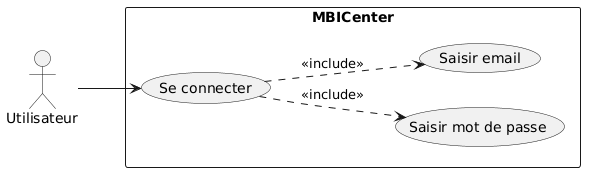
\includegraphics[width=0.7\textwidth]{project/images/RP2n3e9038Pt4jwXOOS4sGmXH2S79yC3D4V59iUTkIkJyTszYeD4r__x-ZTj7mM3BBFDipopT1KG3u6dcy38WOomTuhGY0ym25kEABG43VDC3NIJ9IZEXzEHd50euA48O8baC2Pq8J3UkUGgnGZ3iOQjWHmvmEpJMe8xHWrNS_TFf1dPVeGc2Uj2hQsgJeTW3stBpjXbfAxRmkONlYkUsl.png}
    \caption{Diagramme de cas d'utilisation "authentification"}
    \label{fig:usecase_login}
\end{figure}

\noindent Le tableau \ref{tab:authentification} présente la description textuelle du cas d’utilisation «Authentification».
\vspace{0.3cm} % petit espace avant le tableau

\small % optionnel : réduit légèrement la taille du texte du tableau
\begin{longtable}{|l|p{12cm}|}
\caption{Cas d’utilisation –Authentification} \label{tab:authentification} \\
\hline
\textbf{Élément} & \textbf{Description} \\
\hline
\endfirsthead
\hline
\textbf{Élément} & \textbf{Description} \\
\hline
\endhead

Cas d’utilisation & 
\begin{itemize}
    \item Authentification 
\end{itemize} \\
\hline
Acteur & 
\begin{itemize}
    \item Utilisateur
\end{itemize} \\
\hline
Préconditions & 
\begin{itemize}
    \item L'utilisateur possède un compte vérifié et approuvé dans le système

\end{itemize} \\
\hline
Scénario de base & 
1. L’utilisateur saisit  l'email  et le mot de passe \\
& 2. Le système vérifie que les champs ne sont pas vides \\
& 3. Le système vérifie que l’email existe dans la base de données\\
& 4. Le système compare le mot de passe saisi avec le mot de passe hashé\\
& 5.Le système vérifie le statut du compte  \\
& 6. Le système génère un JWT contenant (id,email,role)\\
& 7. Le token est stocké (Cookie sécurisé ou localStorage)\\
& 8. Le système redirige l’utilisateur vers son espace selon son rôle\\
\hline
Scénarios alternatifs & 
\textbf{Champs vides :}
 Le système affiche un message demandant de remplir tous les champs \\
& \textbf{Email inexistant :} Le système affiche un message d’erreur et refuse l’authentification \\
& \textbf{Mot de passe incorrect :} Le système affiche un message d’erreur et permet une nouvelle tentative \\
& \textbf{Compte non autorisé :} Le système bloque l’accès et affiche un message indiquant que le compte n’est pas autorisé \\
\hline
Post-condition & 
\begin{itemize}[leftmargin=*]
    \item Authentification réussie
    \item JWT généré
    \item Accès au dashboard selon le rôle
\end{itemize} \\
\hline
\end{longtable}


\noindent \textbf{Amélioration du cas d'utilisation « modification du mot de passe » :}

\noindent La fonctionnalité de récupération de mot de passe est essentielle pour permettre aux utilisateurs de réinitialiser leur mot de passe en cas d’oubli.
Elle comprend la soumission d’une demande de réinitialisation, la réception d’un lien de réinitialisation envoyé par email, l’accès à ce lien sécurisé, ainsi que la définition d’un nouveau mot de passe.

\noindent La figure \ref{fig:usecase_password_modification} présente le diagramme de cas d’utilisation expliquant le fonctionnement de la modification du mot de passe.
 \begin{figure}[H]
    \centering
    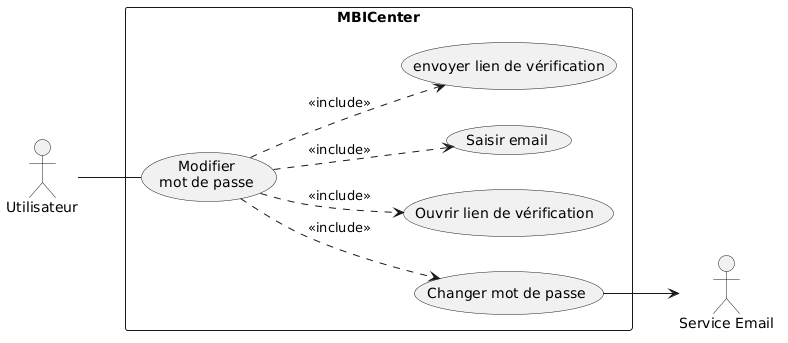
\includegraphics[width=1\textwidth]{project/images/ddcsc.png}
    \caption{Diagramme de cas d'utilisation "modification du mot de passe"}
    \label{fig:usecase_password_modification}
\end{figure}
\noindent Le tableau \ref{tab:password_modification} présente la description textuelle du cas d’utilisation «modification du mot de passe».

\begin{longtable}{|l|p{12cm}|}
\caption{cas d'utilisation-modification du mot de passe}
\label{tab:password_modification} \\
\hline
\textbf{Élément} & \textbf{Description} \\
\hline
\endfirsthead
\hline
\textbf{Élément} & \textbf{Description} \\
\hline
\endhead
Cas d’utilisation & Mot de passe oublié (Forgot Password) \\
\hline
Acteur & Utilisateur \\
\hline

Précondition & 
\begin{itemize}[leftmargin=*]
    \item L’utilisateur a oublié son mot de passe
    \item L’utilisateur possède un compte dans le système
\end{itemize} \\
\hline
Scénario principal & 
\textbf{ Scénario 1: Demande de réinitialisation}
\begin{enumerate}[leftmargin=*]
    \item L’utilisateur clique sur « Mot de passe oublié »
    \item Il saisit son adresse email
    \item Le système vérifie la validité de l’email
    \item Le système vérifie l’existence de l’email en base
    \item Le système envoie un lien de réinitialisation unique et temporaire
    \item Le système affiche un message de confirmation
\end{enumerate}

\textbf{Scénario 2: Réinitialisation du mot de passe}
\begin{enumerate}[leftmargin=*]
    \item L’utilisateur ouvre le lien reçu par email
    \item Il saisit le nouveau mot de passe et sa confirmation
    \item Le système vérifie que les champs sont remplis
    \item Le système vérifie que les mots de passe sont identiques
    \item Le système vérifie la validité du lien (token non expiré)
    \item Le système met à jour le mot de passe (hash)
    \item Le système affiche un message de succès et redirige vers login
\end{enumerate}
\\
\hline
Scénarios alternatifs & 
\begin{itemize}[leftmargin=*]
    \item \textbf{Email invalide ou vide :} le système affiche un message d’erreur et bloque l’envoi
    \item \textbf{Email inexistant :} affichage d’un message générique pour des raisons de sécurité
    \item \textbf{Mots de passe non identiques :} le système rejette la demande
    \item \textbf{Lien expiré ou déjà utilisé :} le système affiche une erreur et demande une nouvelle réinitialisation
\end{itemize}
\\
\hline

Postcondition & 
\begin{itemize}[leftmargin=*]
    \item Un lien de réinitialisation est généré
    \item Un email est envoyé à l’utilisateur
    \item L’utilisateur accède au formulaire de réinitialisation
    \item Le mot de passe est mis à jour dans la base de données
    \item L’utilisateur peut se reconnecter avec le nouveau mot de passe
\end{itemize}
\\
\hline
\end{longtable}

\subsection{Conception}
La phase de conception modélise techniquement le fonctionnement de l'authentification à l'aide de diagrammes de séquence. Ils illustrent chronologiquement les interactions entre l'utilisateur et le système pour garantir la sécurité des flux, depuis l'inscription de l'apprenant jusqu'à sa validation finale par l'administration.
\vspace{0.3cm}

\noindent\textbf{Diagramme de séquence : Inscription de l'apprenant}

\noindent Ce diagramme illustre le processus de création d'un nouveau compte sur la plateforme. L'utilisateur fournit ses donnés personnelles. La figure \ref{cap:inscription_apprenant} presente comment le système procède d'abord à une vérification du format des données et l'unicité de l'email. Une fois validé, le mot de passe est haché et le compte est créé avec un statut "non vérifié". Un lien de confirmation est alors envoyé par email à l'utilisateur pour confirmer l'identité de l'apprenant.

\vspace{0.3cm}
\noindent \textbf{Diagramme de séquence : Vérification de l'adresse email}

\noindent Ce diagramme démontre la validation de l'email,comme il est représenté dans la Figure \ref{cap:usecase_seq_verif}, faisant passer le compte du statut "non vérifié" à "en attente". En cliquant sur le lien reçu, l'apprenant transmet un code de sécurité que le système vérifie (intégrité et validité). Une fois l'email confirmé, le profil est prêt pour l'étape finale : l'examen et la validation manuelle par l'administrateur.

\vspace{0.3cm}
\noindent\textbf{Diagramme de séquence : Login}

\noindent Le processus d’authentification est  détaillé en deux scénarios spécifiques : le login de l’apprenant et celui du responsable, afin de distinguer les différents parcours d’accès selon le rôle de l’utilisateur.

\newpage
\thispagestyle{empty}

\begin{figure}[H]
\centering

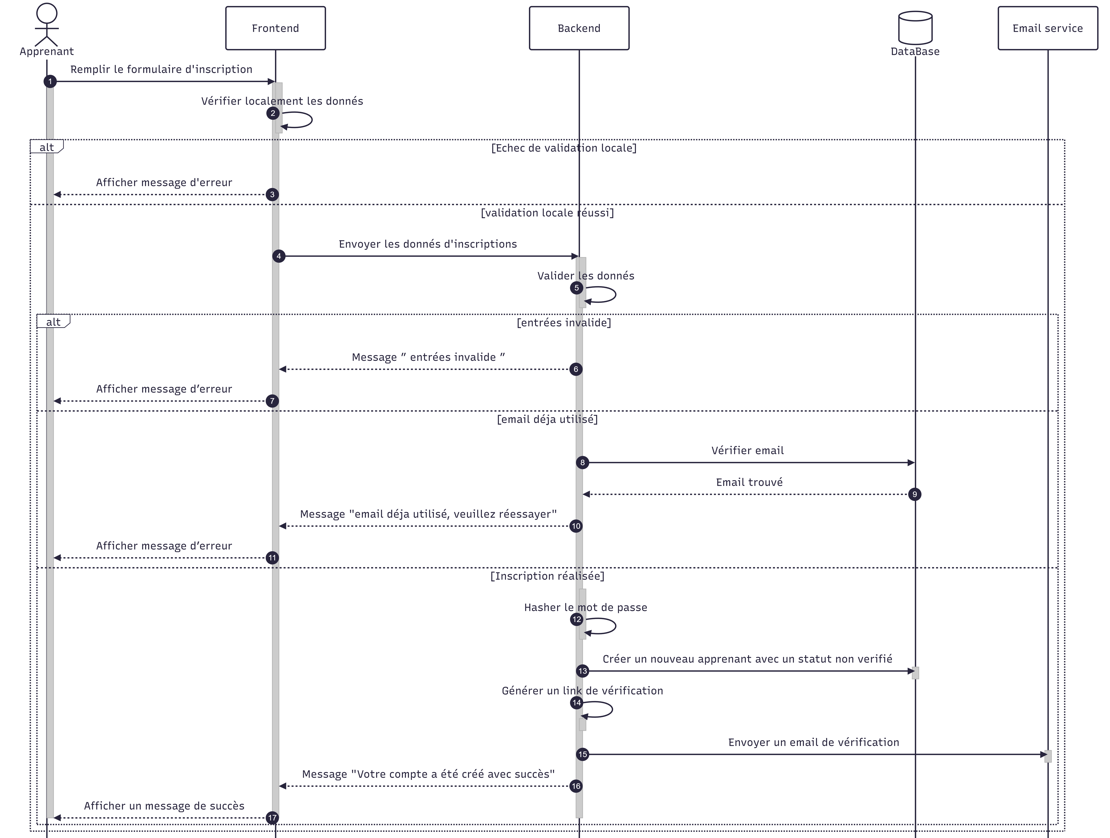
\includegraphics[height=0.45\textheight,keepaspectratio]{project/images/inscds.png}

\caption{Diagramme de séquence <<Inscription de l'apprenant>>}
\label{cap:inscription_apprenant}

\end{figure}

\begin{figure}[H]
  \centering
    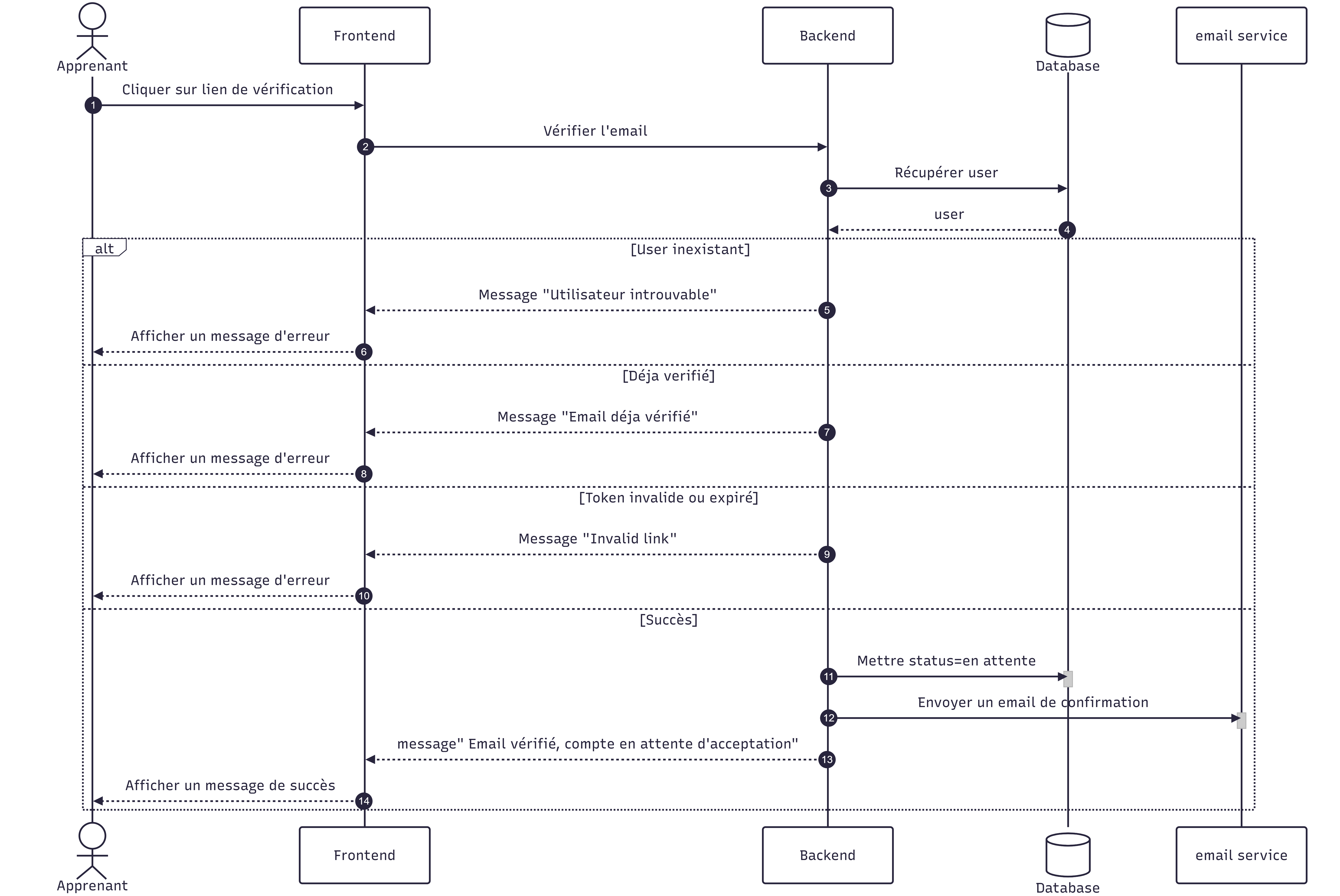
\includegraphics[width=\textwidth,height=0.9\textheight,keepaspectratio]{project/images/Verify-mail.png}
  \caption{Diagramme de séquence <<Vérification de l'adresse email>> }
  \label{cap:usecase_seq_verif}
\end{figure}


\vspace{0.3cm}

\noindent \textbf{Diagramme de séquence: Login -Apprenant}

\noindent le diagramme décrit la procédure de connexion sécurisée pour le profil apprenant, qui est schématisé dans la Figure \ref{cap:Diagramme de séquence <<Login - Apprenant>>}.
\vspace{0.3cm}

\begin{figure}[H]
  \centering
    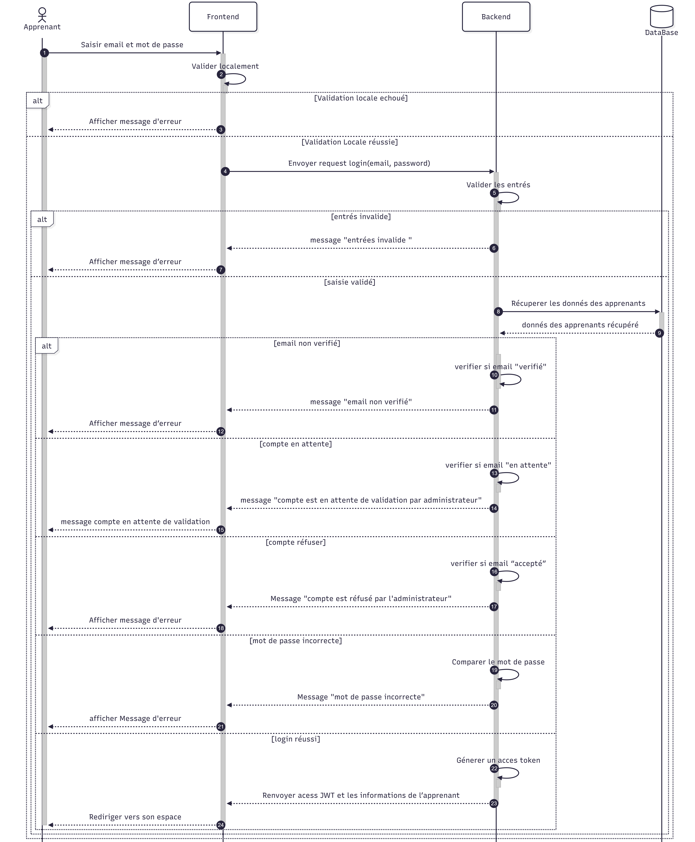
\includegraphics[scale=0.9]{project/images/loginds.png}
  \caption{Diagramme de séquence <<Login - Apprenant>> }
  \label{cap:Diagramme de séquence <<Login - Apprenant>>}
\end{figure}
\newpage
\noindent \textbf{Diagramme de séquence : Login -Responsables et Administrateurs}

\noindent Le diagramme exposé dans la Figure \ref{cap:Diagramme de séquence <<Login -Responsables et Administrateurs>>}, présente le flux d’authentification pour les profils administratifs, tels que le Directeur, le Responsable pédagogique , Responsable financier ou l’Administrateur. Bien que ces utilisateurs possèdent des niveaux d’accès différents, leurs étapes de connexion sont identiques, ce qui justifie la conception d’un diagramme unifié.



\begin{figure}[H]
  \centering
    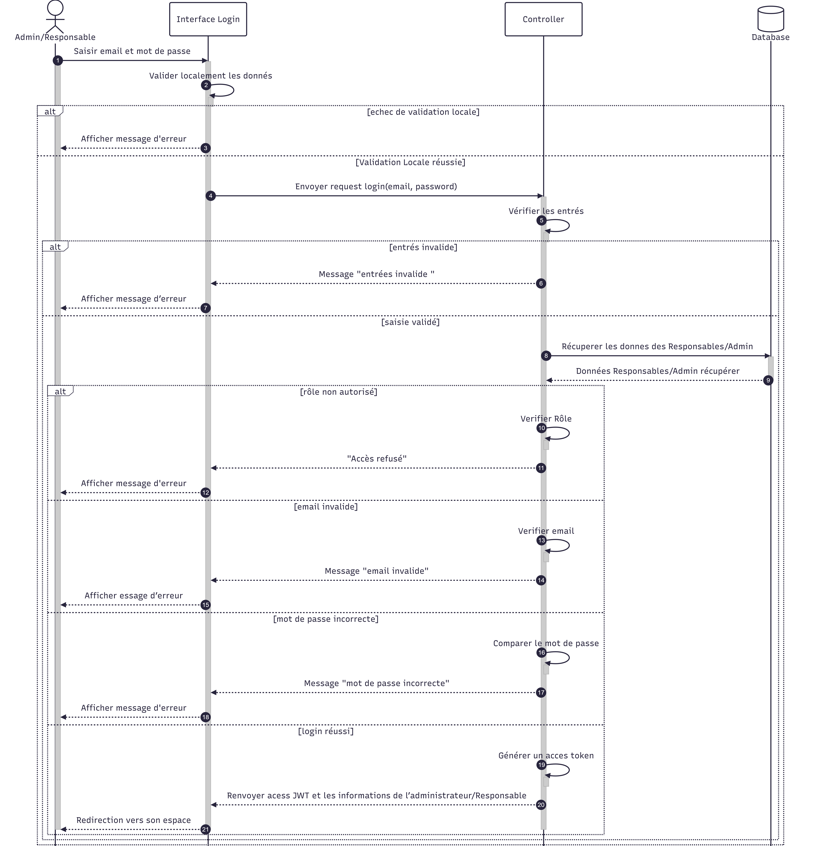
\includegraphics[scale=0.8]{project/images/LoginResds.png}
  \caption{Diagramme de séquence <<Login -Responsables et Administrateurs>> }
  \label{cap:Diagramme de séquence <<Login -Responsables et Administrateurs>>}
  \centering
\end{figure}

\newpage
\noindent\textbf{Diagramme de séquence: Mot de passe oublié}

\noindent Ce diagramme modelise la demande de récupération de compte. Après avoir vérifié l'existence de l'utilisateur, le système lui envoie un lien de réinitialisation temporaire par email comme il est représenter dans la Figure \ref{cap:Diagramme de séquence <<Mot de passe oublié>>}. Ce mécanisme sécurisé garantit que seul le propriétaire légitime de la boîte mail peut initier la modification de son mot de passe.
\vspace{0.5cm}
\begin{center}
  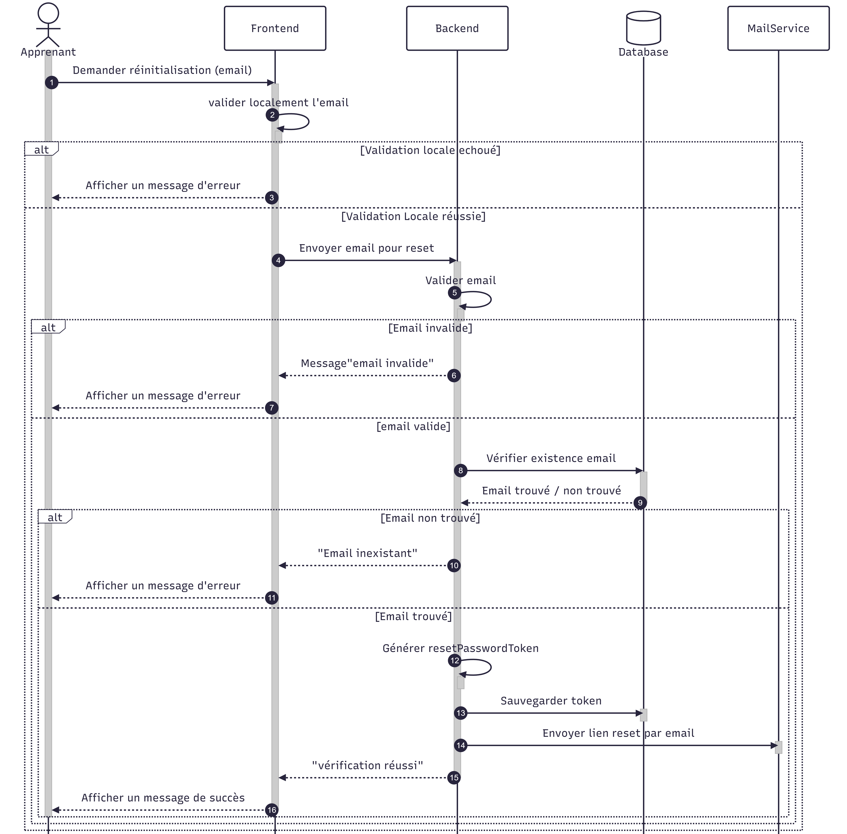
\includegraphics[width=1.1\textwidth,keepaspectratio]{project/images/forgetpassds.png}
  \captionof{figure}{Diagramme de séquence <<Mot de passe oublié>>}
  \label{cap:Diagramme de séquence <<Mot de passe oublié>>}
\end{center}
\newpage
\noindent\textbf{Diagramme de séquence : Vérification de lien de réinitialisation}

Ce diagramme décrit la validation automatique du lien envoyé par email. Avant d'autoriser tout changement, le système vérifie si le lien utilisé est toujours fonctionnel. Cela permet de bloquer la procédure si le lien a expiré, évitant ainsi à l'utilisateur de perdre du temps avec un lien expiré comme illustré dans la Figure \ref{cap:usecase_seq_linkReset}.

\begin{figure}[H]
  \centering
    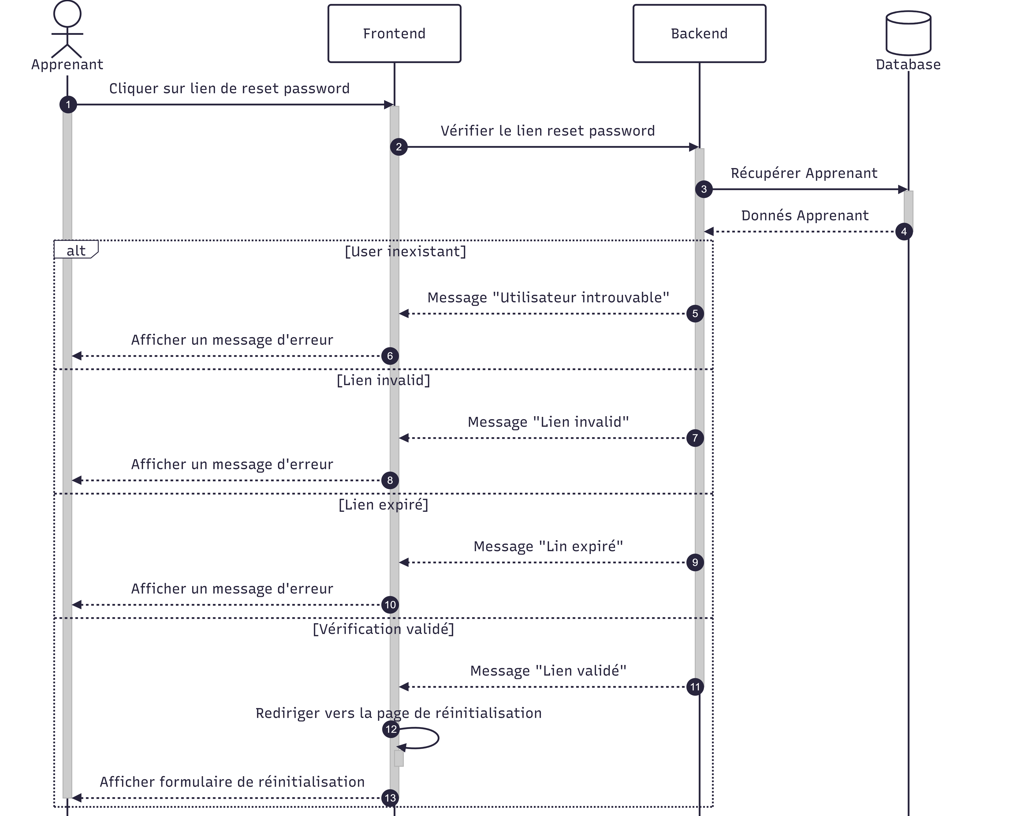
\includegraphics[width=1.1\textwidth,height=0.9\textheight,keepaspectratio]{project/images/linkressds.png}
  \caption{Diagramme de séquence <<Vérification du lien de réinitialisation>> }
  \label{cap:usecase_seq_linkReset}
\end{figure}

\vspace{0.3cm}

\noindent\textbf{Diagramme de séquence : Réinitialisation du mot de passe}

\noindent Ce dernier diagramme schématisé dans la Figure \ref{cap:Diagramme de séquence:<<Réinitialisation du mot de passe>>} présente la mise à jour finale du mot de passe. L’utilisateur saisit ses nouvelles informations, qui sont envoyées de manière  sécurisée au système. Après une vérification finale de la demande, le système sécurise le nouveau mot de passe et l’enregistre dans la base de données.
\newpage
\begin{figure}[H]
  \centering
    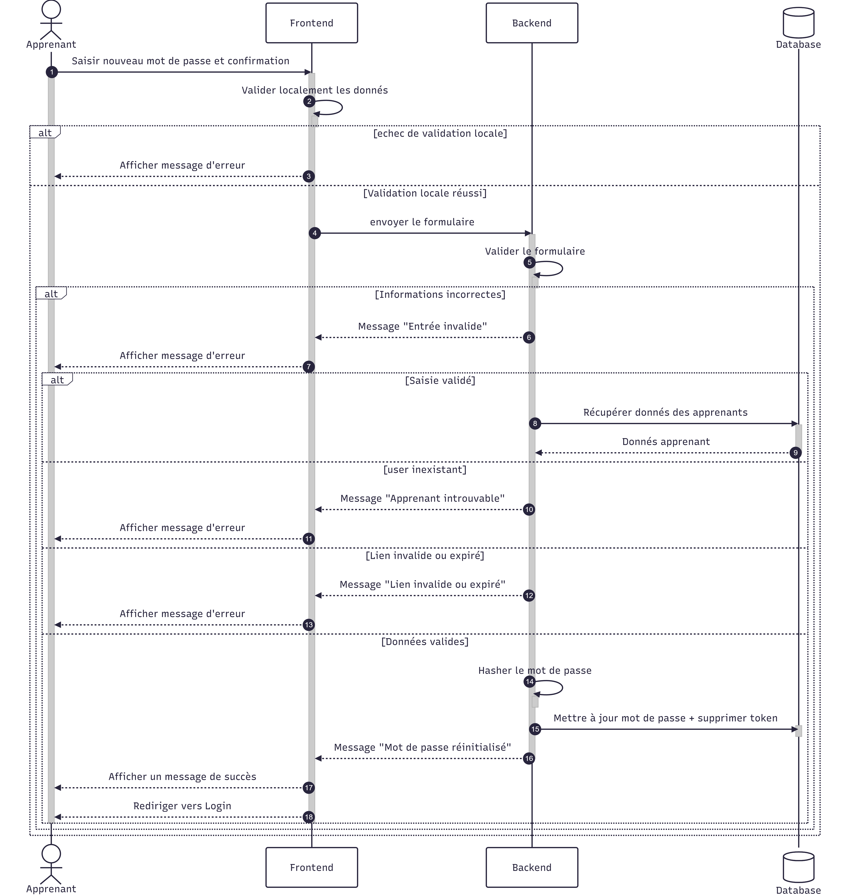
\includegraphics[width=1.1\textwidth,height=1\textheight,keepaspectratio]{project/images/newpassds.png}
  \caption{Diagramme de séquence <<Réinitialisation du mot de passe>> }
  \label{cap:Diagramme de séquence:<<Réinitialisation du mot de passe>>}
\end{figure}




\newpage
\subsection{Réalisation}
Cette section présente les interfaces de l'authentification. Nous allons détailler les différents modules en mettant l’accent sur l’expérience utilisateur et les fonctionnalités implémentées.

\vspace{0.3cm}
\noindent\textbf{Interface d'inscription}

\noindent La première étape pour l'apprenant est de renseigner ses informations de base via une interface intuitive. Comme l'illustre la Figure \ref{cap:Interface d'inscription:standard}, le formulaire comprend des champs obligatoires avec une aide à la saisie pour guider l'apprenant. La figure \ref{cap:Interface d'inscription:champs-vide} montre comment l'interface réagit lorsque les données ne respectent pas le format attendu (par exemple, un mot de passe trop simple ou un email mal formé). Si un utilisateur tente de s'inscrire avec un email déjà existant, une alerte spécifique est déclenchée comme le montre la figure \ref{cap:Interface d'inscription:champs-invalide}.

\begin{center}


\begin{minipage}{0.9\textwidth}
    \centering
    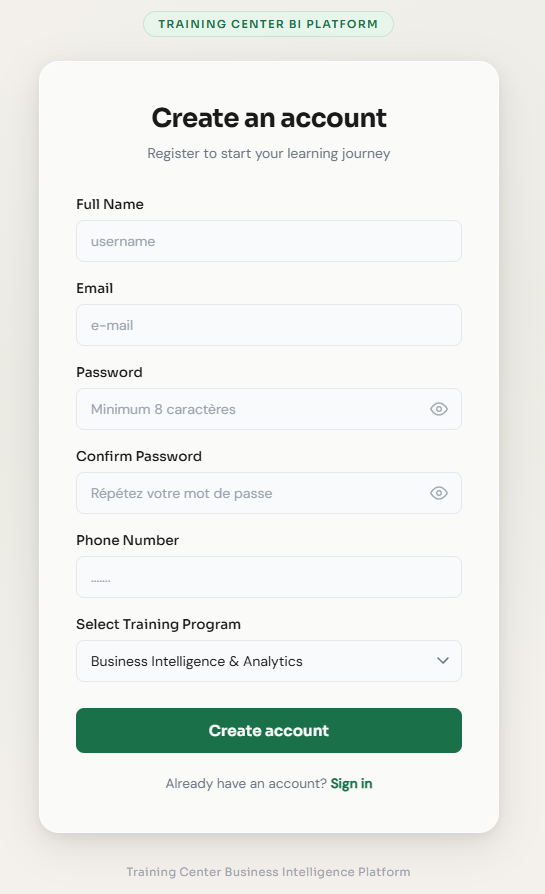
\includegraphics[width=1\linewidth]{project/images/register-cap.png}
    \captionof{figure}{Interface d'inscription : standard}
    \label{cap:Interface d'inscription:standard}
\end{minipage}

\begin{minipage}{0.45\textwidth}
    \centering
    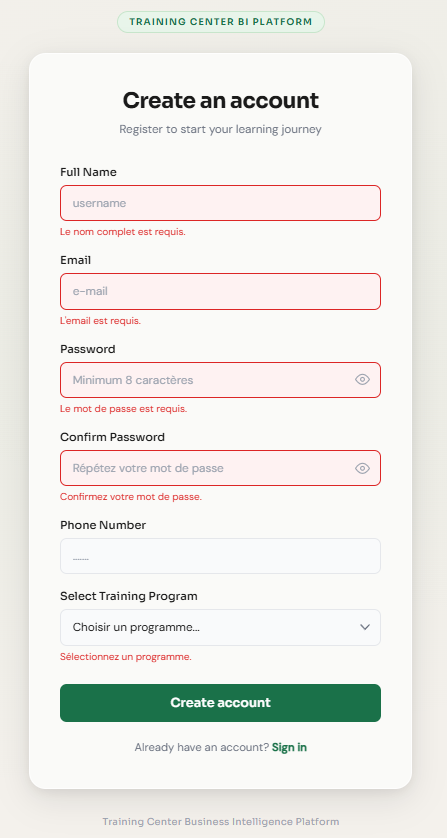
\includegraphics[width=0.9\linewidth]{project/images/register-empty.png}
    \captionof{figure}{Interface d'inscription : champs vides}
    \label{cap:Interface d'inscription:champs-vide}
\end{minipage}
\hfill
\begin{minipage}{0.45\textwidth}
    \centering
    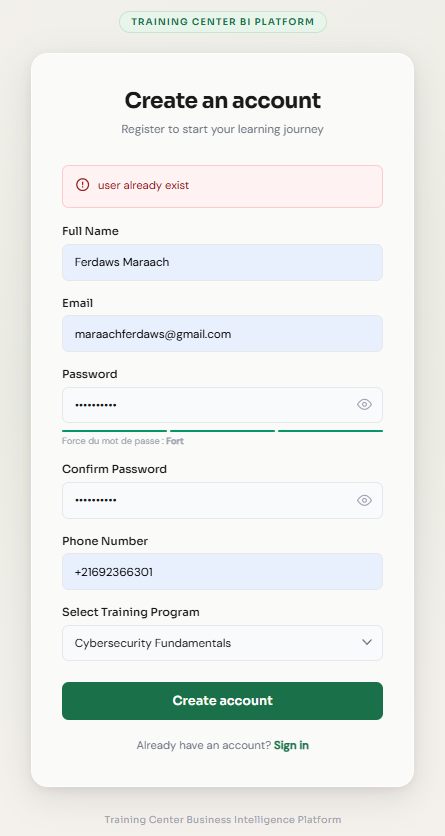
\includegraphics[width=0.9\linewidth]{project/images/register-invalid.png}
    \captionof{figure}{Interface d'inscription : champs invalides}
    \label{cap:Interface d'inscription:champs-invalide}
\end{minipage}

\vspace{0.4cm}



\end{center}

\FloatBarrier

\newpage
\noindent \textbf{Étape de la Vérification d'email}

\noindent L’interface illustrée en Figure \ref{cap:interface d'inscription: vérifier email} informe l'utilisateur qu'un lien de confirmation a été envoyé à son adresse mail pour valider son compte. À cette étape, la Figure \ref{cap:interface d'inscription: email de vérification}  présente le contenu du mail reçu par l'utilisateur, incluant un bouton sécurisé contenant un token d'activation. 

\noindent Dans le cas où l'utilisateur clique sur un lien déjà utilisé ou dont la durée de validité est dépassée, l’interface de la \ref{cap:interface d'inscription:lien non valide} s'affiche pour lui proposer de renvoyer un nouvel email de vérification.

\noindent Enfin, comme le montre la Figure \ref{cap:interface d'inscription:inscription vérifié}, une page de confirmation apparaît brièvement suite à une validation réussie, avant de rediriger automatiquement l'utilisateur vers la page de connexion.



\begin{center}
    \centering
    
    % الصف الأول
    \begin{minipage}{0.45\textwidth}
        \centering
        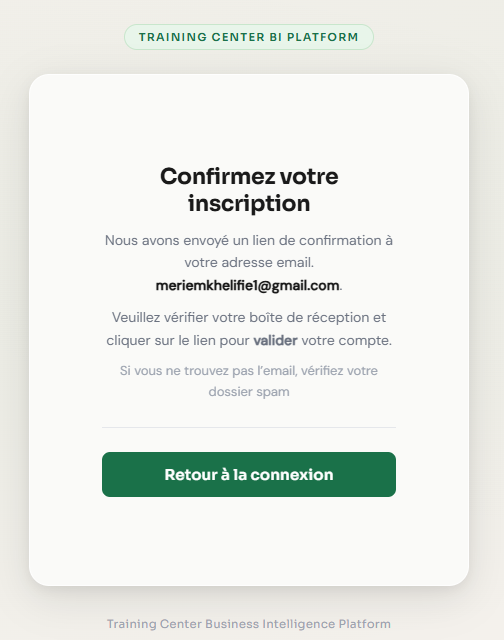
\includegraphics[width=1\linewidth]{project/images/confirme.png}
        \captionof{figure}{interface d'inscription : vérifier email}
        \label{cap:interface d'inscription: vérifier email}
    \end{minipage}
    \hfill
    \begin{minipage}{0.45\textwidth}
        \centering
        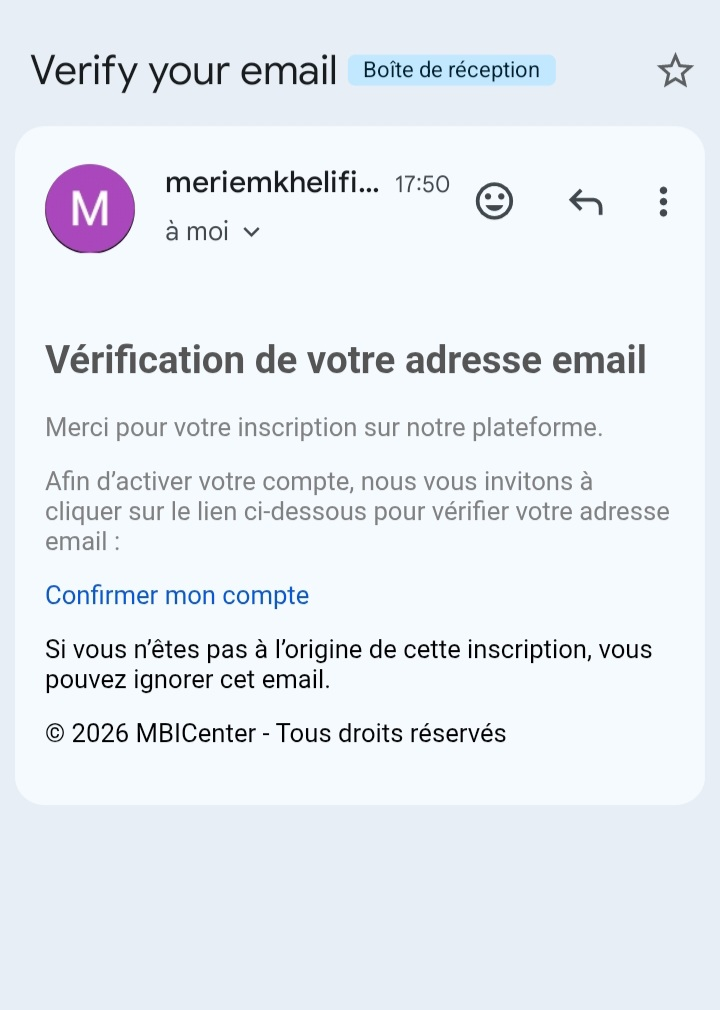
\includegraphics[width=0.8\linewidth]{project/images/email.verify.jpeg}
        \captionof{figure}{interface d'inscription : email de vérification}
        \label{cap:interface d'inscription: email de vérification}
    \end{minipage}
    
    \vspace{0.5cm}
    
    % الصف الثاني
    \begin{minipage}{0.45\textwidth}
        \centering
        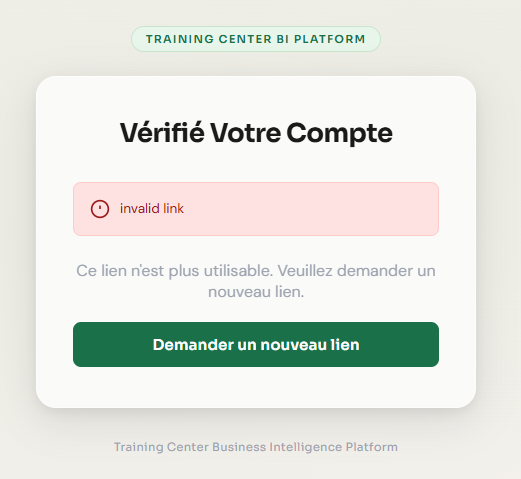
\includegraphics[width=1\linewidth]{project/images/lien-invalide.png}
        \captionof{figure}{interface d'inscription : lien non valide}
        \label{cap:interface d'inscription:lien non valide}
    \end{minipage}
    \hfill
    \begin{minipage}{0.45\textwidth}
        \centering
        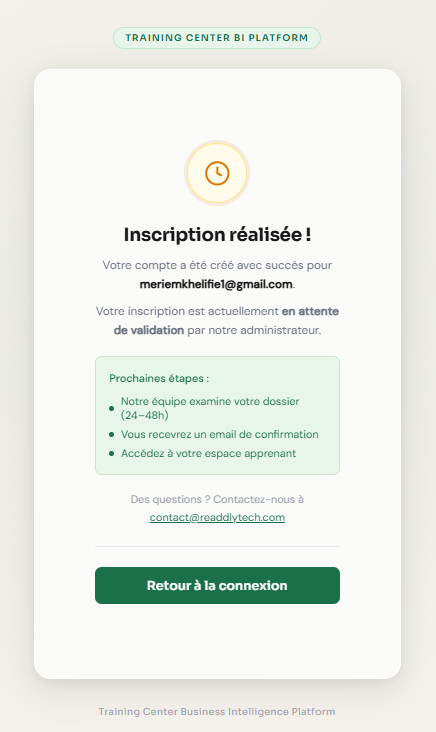
\includegraphics[width=0.8\linewidth]{project/images/validé.png}
        \captionof{figure}{interface d'inscription : inscription vérifié}
        \label{cap:interface d'inscription:inscription vérifié}
    \end{minipage}

\end{center}

\newpage
\noindent\textbf{Interface Login:}

\noindent L’interface de connexion dans la Figure \ref{fig:Interface login:état normale}  constitue le point d’entrée unique pour tous les utilisateurs. Afin de sécuriser l'accès, un message d’erreur s’affiche en cas d’identifiants incorrects comme la montre Figure \ref{cap:Interface login: données invalide}. Le système vérifie également le statut du compte : les profils en attente de validation illustré dans la Figure \ref{cap:Interface login:Apprenant ena attente d'acceptation} ou rejetés, représenté dans la Figure \ref{cap:Interface login:Apprenant-est-refusé} sont informés par des interfaces spécifiques. Par ailleurs, si le compte est désactivé, l’accès est refusé et un message d’erreur dédié est affiché, comme le montre la Figure \ref{cap:Interface login: Utilisateur désactivé}. Une fois l'authentification réussie, la plateforme redirige automatiquement l'utilisateur vers un espace selon son rôle.


\begin{figure}[H]
  \centering
    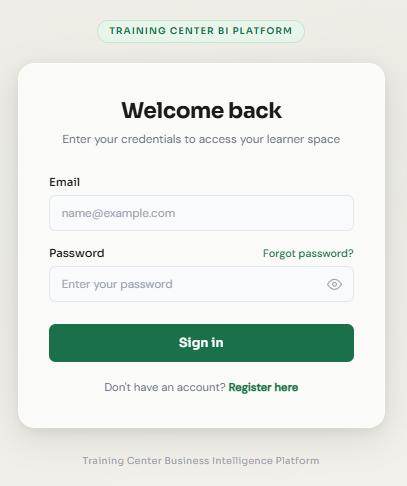
\includegraphics[width=1\linewidth]{project/images/login.png}
  \caption{ Interface login : état normale}
  \label{fig:Interface login:état normale}
\end{figure}

\begin{center}
    \centering
    
    % الصف الأول
    \begin{minipage}{0.45\textwidth}
        \centering
        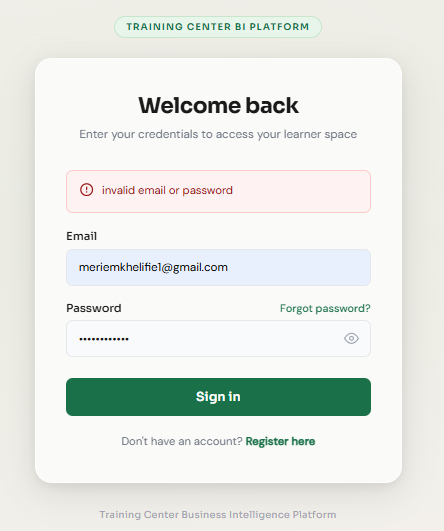
\includegraphics[width=0.9\linewidth]{project/images/Login-invalide.png}
        \captionof{figure}{Interface login : données invalide}
        \label{cap:Interface login: données invalide}
    \end{minipage}
    \hfill
    \begin{minipage}{0.5\textwidth}
        \centering
        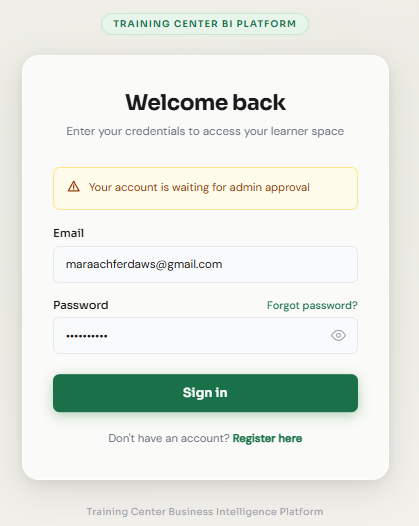
\includegraphics[width=0.79\linewidth]{project/images/en attente.png}
        \captionof{figure}{Interface login : Apprenant en attente d'acceptation}
        \label{cap:Interface login:Apprenant ena attente d'acceptation}
    \end{minipage}
\end{center}
    \vspace{0.5cm}
    % الصورة في الوسط
\begin{center}
    \centering  
    \begin{minipage}{0.45\textwidth}
        \centering
        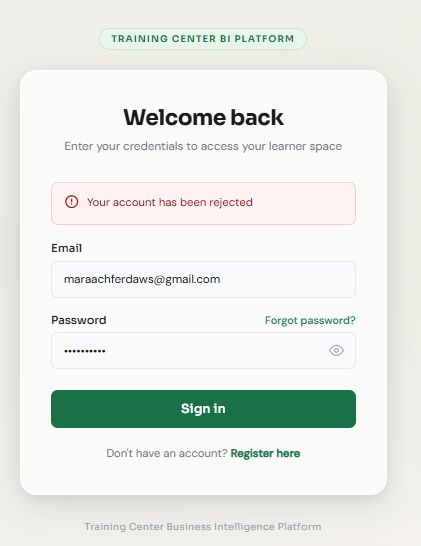
\includegraphics[width=0.9\linewidth]{project/images/rejected.png}
        \captionof{figure}{Interface login : Apprenant est refusé}
        \label{cap:Interface login:Apprenant-est-refusé}
    \end{minipage}
    \hfill
    \begin{minipage}{0.45\textwidth}
        \centering
        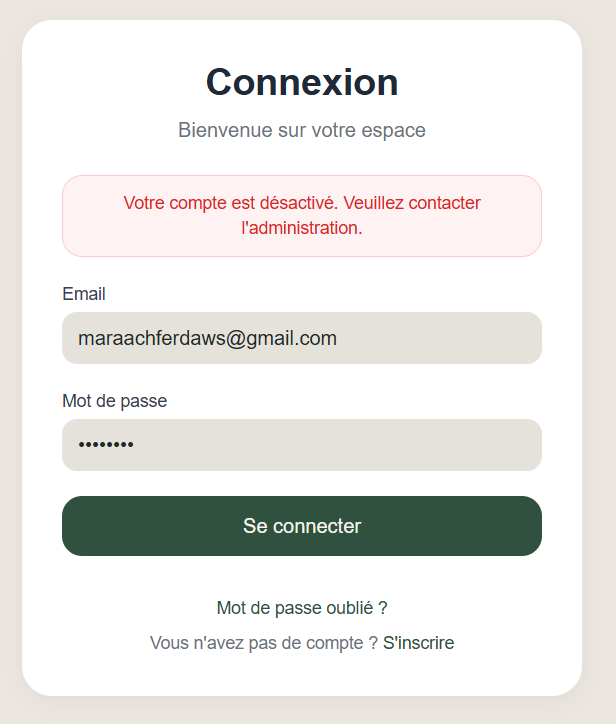
\includegraphics[width=0.9\linewidth]{project/images/compte-désactivé.png}
        \captionof{figure}{Interface login : Utilisateur désactivé}
        \label{cap:Interface login: Utilisateur désactivé}
    \end{minipage}
\end{center}







\noindent \textbf{Interface Réinitialisation du mot de passe:}

\noindent L’interface illustrée en Figure \ref{cap:R_mp} permet à l'utilisateur de saisir son adresse email pour initier la procédure.
Si l'adresse saisie ne correspond à aucun compte enregistré ou si le format est incorrect, l'interface de la Figure \ref{cap:F_F} s'affiche.

\vspace{0.8cm}

\begin{figure}[H]
  \centering
    \centering
        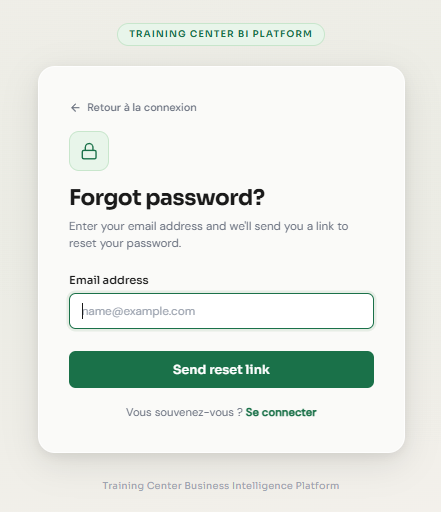
\includegraphics[width=\linewidth]{project/images/forgot-pass.png}
        \captionof{figure}{Interface de réinitialisation du mot de passe }
        \label{cap:R_mp}
\end{figure}


\begin{figure}[H]
    \centering
        \centering
        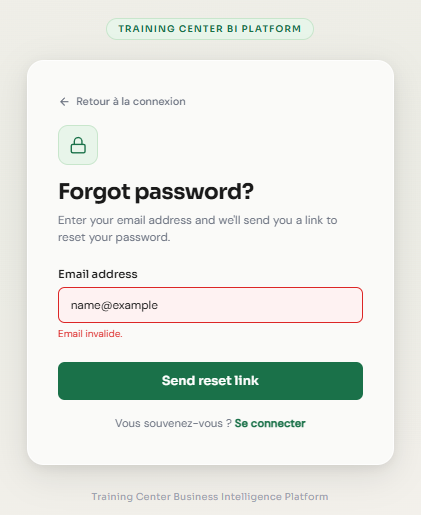
\includegraphics[width=0.5\linewidth]{project/images/pass-invalide.png}
        \captionof{figure}{Interface de réinitialisation : email invalide}
        \label{cap:F_F}
\end{figure}


\noindent \textbf{interface de lien de vérification :}

\noindent Une fois un email valide soumis comme le montre la figure \ref{cap:Interface réinitialisation: email }  , l'interface de la Figure \ref{cap:Interface de réinitialisation:email de réinitialisation} informe l'utilisateur qu'un lien de réinitialisation lui a été envoyé. Cette étape confirme la prise en compte de la demande par le serveur.

\noindent En accédant à ce lien, l’utilisateur est redirigé vers une interface dédiée à la réinitialisation du mot de passe, comme le montre la figure \ref{cap:Interface de réinitialisation:etat}, où il peut saisir un nouveau mot de passe.

\noindent Le lien envoyé par email a une durée de validité limitée. Si l'utilisateur clique sur un lien obsolète ou déjà utilisé, l'interface présentée en Figure \ref{cap:Interface de réinitialisation: lien invalide} apparaît, l'invitant à renouveler sa demande.

 \begin{center}
    \centering  
    \begin{minipage}{0.45\textwidth}
        \centering
        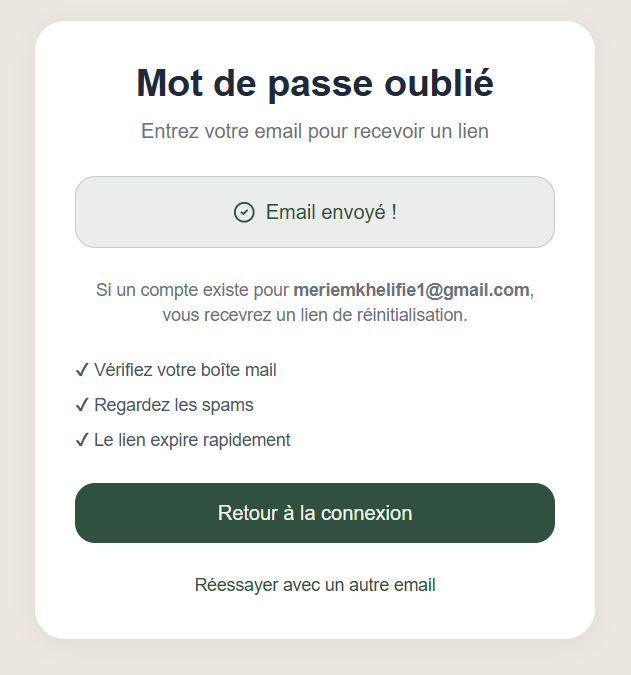
\includegraphics[width=0.9\linewidth]{project/images/pas-mail.png}
        \captionof{figure}{Interface de réinitialisation : email envoyé}
        \label{cap:Interface réinitialisation: email }
    \end{minipage}
    \hfill
    \begin{minipage}{0.45\textwidth}
        \centering
        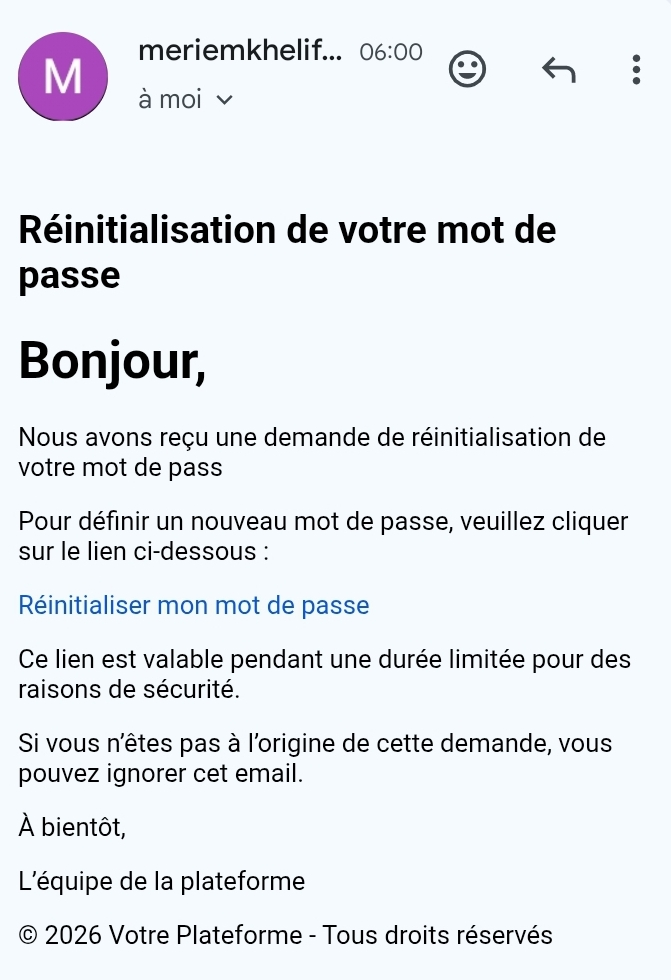
\includegraphics[scale=0.23]{project/images/email-reset.jpeg}
        \captionof{figure}{Interface de réinitialisation : email de réinitialisation}
        \label{cap:Interface de réinitialisation:email de réinitialisation}
    \end{minipage}
\end{center}

    
  
    
  
 \begin{center}   
    % الصف اللي لتحت (زوز صور)
    \begin{minipage}{0.45\textwidth}
        \centering
        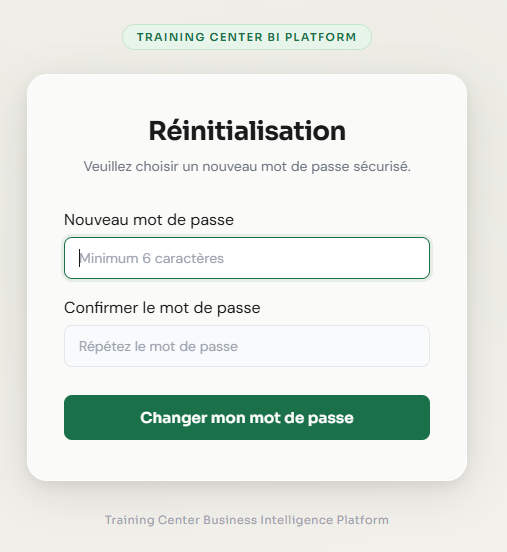
\includegraphics[width=\linewidth]{project/images/reset-pass.png}
        \captionof{figure}{Interface de réinitialisation : état normale}
        \label{cap:Interface de réinitialisation:etat}
    \end{minipage}
    \hfill
    \begin{minipage}{0.45\textwidth}
        \centering
        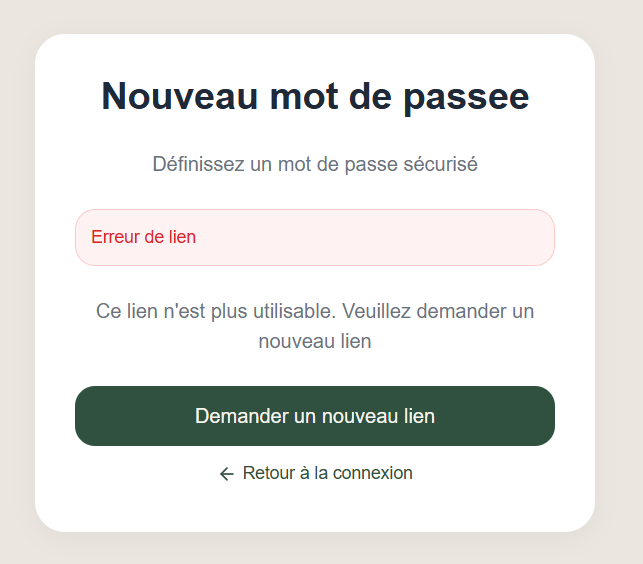
\includegraphics[width=\linewidth]{project/images/invalid-link.png}
        \captionof{figure}{Interface de réinitialisation : lien invalide}
        \label{cap:Interface de réinitialisation: lien invalide}
    \end{minipage}

\end{center}

\vspace{0.5cm}
\noindent \textbf{Interface de création du nouvelle mot de passe:}

\noindent Si le lien est valide, l'utilisateur accède au formulaire de la Figure \ref{cap:reset_form}. Cette interface sécurisée permet de saisir et de confirmer le nouveau mot de passe.
Le système applique également des règles de validation afin de garantir la robustesse du mot de passe. Ainsi, si le mot de passe saisi ne respecte pas les contraintes définies, un message d’erreur s’affiche à l’écran, comme illustré dans la figure \ref{cap:reset_invalid}, invitant l’utilisateur à corriger sa saisie.

\noindent Enfin, après la validation du nouveau mot de passe, un message de succès s'affiche dans la figure \ref{cap:reset_success} et le système redirige automatiquement l'utilisateur vers la page de connexion pour s'authentifier.


\begin{center}
    \centering
    
    % الصف الأول (زوز صور)
    \begin{minipage}{0.45\textwidth}
        \centering
        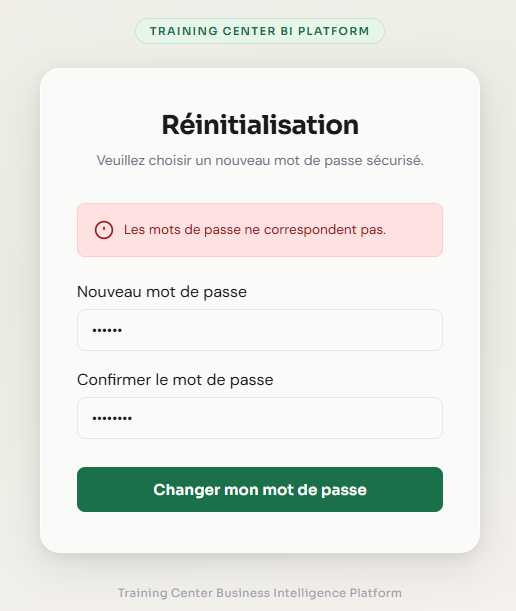
\includegraphics[width=1\linewidth]{project/images/reset-empty.png}
        \captionof{figure}{Interface de réinitialisation : changer le mot de passe}
        \label{cap:reset_form}
    \end{minipage}
    \hfill
    \begin{minipage}{0.45\textwidth}
        \centering
        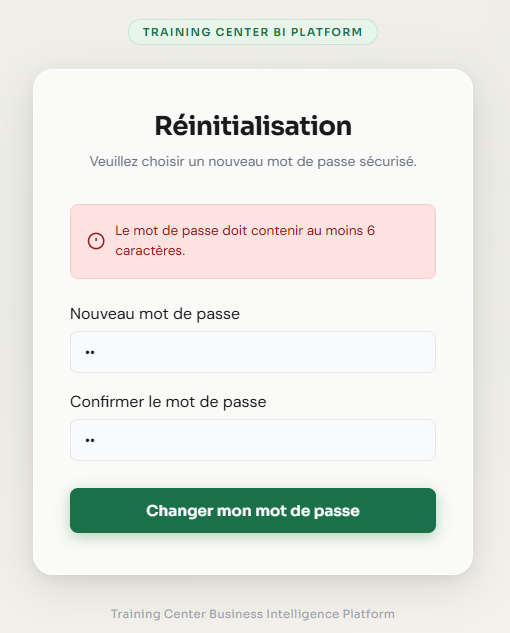
\includegraphics[width=1\linewidth]{project/images/ress-invalide.png}
        \captionof{figure}{Interface de réinitialisation : mot de passe invalide}
        \label{cap:reset_invalid}
    \end{minipage}
    
    \vspace{0.5cm} % espace بين الصفوف
    
    % الصف الثاني (صورة وحدة في الوسط)
    \begin{minipage}{0.7\textwidth}
        \centering
        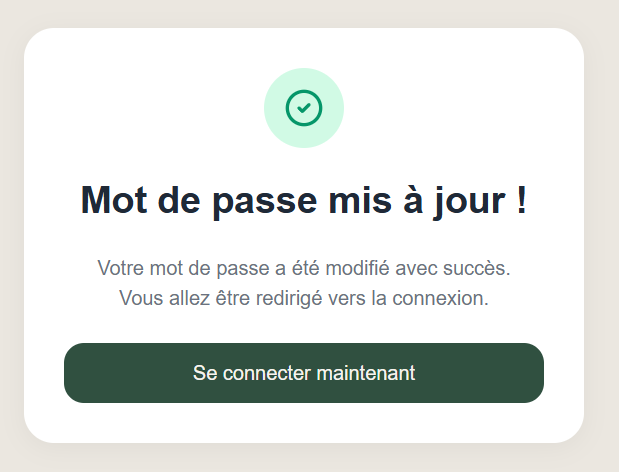
\includegraphics[width=0.8\linewidth]{project/images/ress-success.png}
        \captionof{figure}{Interface de réinitialisation : mot de passe réinitialisé avec succès}
        \label{cap:reset_success}
    \end{minipage}
\end{center}


\section{Sprint 2: Gestion des utilisateurs}
\label{sec:sprint2-gestion-utilisateurs}
Le sprint 2 est consacré au développement du module de gestion des utilisateurs, une fonctionnalité essentielle de notre système.
Ce module permet aux administrateurs de gérer efficacement l’ensemble des utilisateurs de la plateforme, notamment à travers la consultation, la validation (acceptation ou refus), la suppression ainsi que la mise à jour de leurs informations.
L’objectif de ce sprint est de mettre en place une interface intuitive, ergonomique et sécurisée, offrant une gestion complète et centralisée des comptes utilisateurs, afin de répondre aux besoins d’administration du système.
\subsection{Le backlog du sprint 2}
Le backlog du Sprint 2, consigné dans le Tableau \ref{tab:backlog_sprint2}, recense les fonctionnalités de gestion des utilisateurs à développer. Il fournit ainsi un cadre structuré pour l'ordonnancement et le suivi des tâches de cette itération.
\nopagebreak

\begin{table}[H]
\caption{Backlog - Gestion des utilisateurs}
\label{tab:backlog_sprint2}
\centering
\small
\setlength{\tabcolsep}{3pt}
\renewcommand{\arraystretch}{0.85}

\begin{tabular}{|c|>{\centering\arraybackslash}p{2.8cm}|p{9cm}|c|}
\hline
\textbf{ID} & \textbf{Fonctionnalité} & \textbf{User Stories} & \textbf{Priorité} \\
\hline
\multirow{6}{*}{2} & \multirow{6}{=}{\small Gestion des utilisateurs} 
& En tant qu'administrateur, je veux consulter la liste des utilisateurs afin de gérer les comptes & M \\ \cline{3-4}
& & En tant qu'administrateur, je veux modifier les informations d'un utilisateur afin de maintenir les données à jour & M \\ \cline{3-4}
& & En tant qu'administrateur, je veux supprimer un utilisateur afin de retirer les comptes inutiles & M \\ \cline{3-4}
& & En tant qu'administrateur, je veux approuver ou refuser les demandes afin de contrôler l'accès & M \\ \cline{3-4}
& & En tant qu'administrateur, je veux ajouter un nouvel utilisateur afin de créer des comptes & S \\ \cline{3-4}
& & En tant qu'administrateur, je veux activer ou désactiver un utilisateur afin de gérer son statut & S \\
\hline
\end{tabular}

\end{table}

\subsection{Analyse}
L'analyse du module de gestion des utilisateurs nous a permis d'identifier les besoins fonctionnels et de définir précisément les interactions attendues entre l'administrateur et le système
\vspace{0.3cm}

\noindent\textbf{Amélioration du cas d’utilisation « gestion des utilisateurs »:}
 
\noindent Le cas d'utilisation « gestion des utilisateurs » permet à l’administrateur d'effectuer toutes les opérations nécessaires à la gestion efficace des comptes utilisateurs au sein du système.
\vspace{0.3cm}

\noindent La figure \ref{fig:usecase_gestion_utilisateurs} présente le diagramme de cas d'utilisation illustrant les différents scénarios de gestion des utilisateurs, et détaillant les différentes actions que l’administrateur peut réaliser.
 \begin{figure}[H]
    \centering
    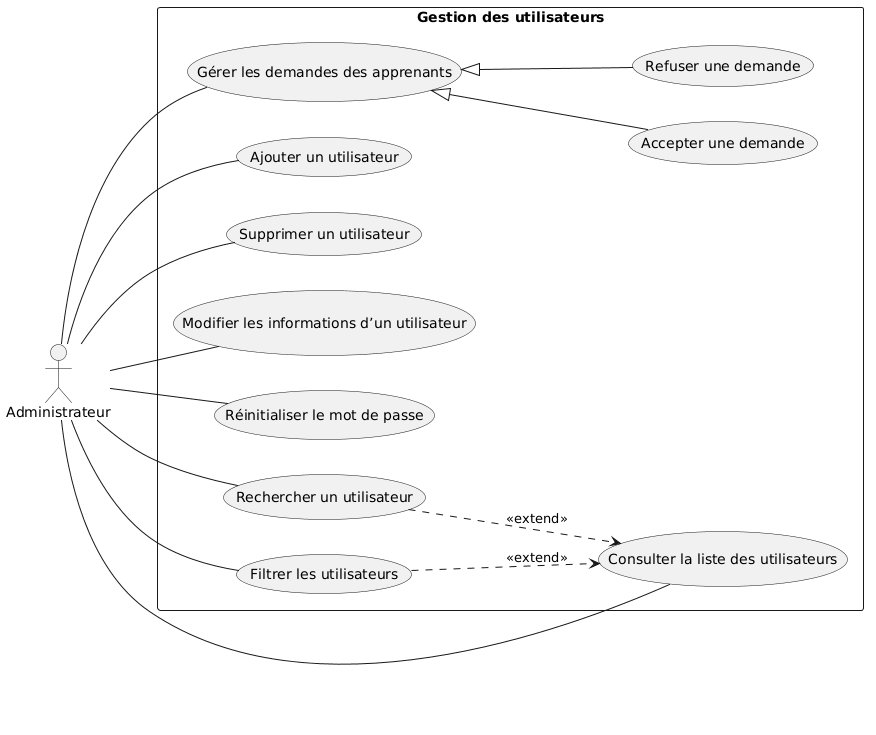
\includegraphics[width=1\textwidth]{project/images/new DG.png}
    \caption{Diagramme de cas d'utilisation "gestion des utilisateurs"}
    \label{fig:usecase_gestion_utilisateurs}
\end{figure}

Le tableau \ref{tab:gestion_utilisateurs} présente la description textuelle du cas d'utilisation « gestion des utilisateurs ».
{\interlinepenalty=10000
\begin{longtable}{|l|p{12cm}|}
\caption{Cas d'utilisation -- Gestion des utilisateurs}
\label{tab:gestion_utilisateurs} \\
\hline
\textbf{Élément} & \textbf{Description} \\
\hline
\endfirsthead
\hline
\textbf{Élément} & \textbf{Description} \\
\hline
\endhead

Cas d'utilisation & Gestion des utilisateurs \\
\hline
Acteur & Administrateur \\
\hline

Préconditions &
L'administrateur est connecté au système (authentifié). \\
& Le système est fonctionnel. \\
& La base de données est accessible. \\
\hline

Scénario de base &
\textbf{Scénario 1 : Consulter la liste des utilisateurs} \\
&- L'administrateur accède à l'interface Gestion des Utilisateurs. \\
&- Le système vérifie la validité du token. \\
&- Le système contrôle que l'utilisateur possède bien le rôle ADMIN. \\
&- Le système renvoie la liste complète des utilisateurs. \\
\\
& \textbf{Scénario 2 : Filtrage des utilisateurs} \\
&- L'administrateur applique un filtre (exemple : Rôle : directeur). \\
&- Le système met à jour dynamiquement le tableau sans rechargement de la page. \\
&- Le système affiche la liste filtrée. \\
\\
& \textbf{Scénario 3 : Rechercher un utilisateur} \\
&- L'administrateur saisit un nom ou un email dans le champ de recherche. \\
&- Le système effectue une recherche en temps réel et met à jour la liste des utilisateurs. \\
&- Le système affiche les résultats correspondants. \\
\\
& \textbf{Scénario 4 : Modifier les informations d'un utilisateur} \\
&- L'administrateur sélectionne un utilisateur dans la liste. \\
&- Le système affiche les détails de l'utilisateur. \\
&- L'administrateur modifie les informations souhaitées. \\
&- Le système met à jour les données de l'utilisateur. \\
\\
& \textbf{Scénario 5 : Ajouter un utilisateur} \\
&- L'administrateur clique sur « Nouvel utilisateur ». \\
&- Le système affiche le formulaire d'ajout. \\
&- L'administrateur renseigne les informations nécessaires (nom, prénom, email, rôle). \\
&- L'administrateur valide la création. \\
&- Le système vérifie la validité des données et l'unicité de l'email. \\
&- Le système hache le mot de passe (bcrypt). \\
&- Le système enregistre le nouvel utilisateur. \\
\\
& \textbf{Scénario 6 : Supprimer un utilisateur} \\
&- L'administrateur sélectionne un utilisateur dans la liste. \\
&- Le système affiche une confirmation de suppression. \\
&- L'administrateur confirme la suppression. \\
\hline
&- Le système supprime l'utilisateur de la base de données. \\
\\
& \textbf{Scénario 7 : Réinitialiser le mot de passe} \\
&- L'administrateur sélectionne un utilisateur. \\
&- Le système envoie un email de réinitialisation à l'utilisateur. \\
&- L'utilisateur saisit un nouveau mot de passe. \\
&- Le système vérifie la validité du mot de passe. \\
&- Le système hache le nouveau mot de passe (bcrypt). \\
&- Le système met à jour les données de l'utilisateur. \\
&- Le système confirme la réussite de l'opération. \\
\\
& \textbf{Scénario 8 : Gérer les demandes des apprenants} \\
&- L'administrateur accède à la section « Apprenants ». \\
&- Le système affiche la liste des apprenants en attente de validation. \\
&- L'administrateur accède à la liste des demandes d'inscription. \\
&- L'administrateur traite la demande (acceptation ou refus). \\
&- Le système met à jour le statut de la demande. \\
&- En cas d'acceptation, le système crée un compte utilisateur pour l'apprenant. \\
&- Le système envoie une notification à l'apprenant. \\
&- En cas de refus, le système archive la demande. \\
\hline

Scénarios alternatifs &
\textbf{Cas 1 -- Échec d'authentification :} Le système détecte un token invalide ou expiré et refuse l'accès. \\
& \textbf{Cas 2 -- Données invalides lors de l'ajout ou modification :} Le système détecte des informations incorrectes ou incomplètes et affiche un message d'erreur. \\
& \textbf{Cas 3 -- Échec d'envoi de l'email de réinitialisation :} Le système ne parvient pas à envoyer l'email et informe l'administrateur de l'échec. \\
\hline

Post-conditions &
\textbf{Scénarios 1, 2 et 3 :} La liste des utilisateurs (complète, filtrée ou recherchée) est affichée à l'administrateur. \\
& \textbf{Scénario 4 :} Les informations de l'utilisateur sélectionné sont mises à jour dans le système. \\
& \textbf{Scénario 5 :} Un nouveau compte utilisateur est créé, le mot de passe est haché et les données sont enregistrées dans la base de données. \\
& \textbf{Scénario 6 :} L'utilisateur sélectionné est définitivement supprimé de la base de données. \\
& \textbf{Scénario 7 :} Un email de réinitialisation est envoyé et le nouveau mot de passe haché est mis à jour dans le système. \\
& \textbf{Scénario 8 :} Le statut de la demande est mis à jour, un compte est créé en cas d'acceptation et une notification est envoyée à l'apprenant. \\
\hline
\end{longtable}
}

\vspace{0.2cm}

\subsection{Conception}
La section Conception présente la modélisation dynamique des principaux scénarios fonctionnels du module de gestion des utilisateurs. Les diagrammes de séquence ci-dessous illustrent, de manière chronologique et détaillée, les interactions entre les différents acteurs du système (Administrateur, Frontend, Backend, Base de données et Serveur Email), en couvrant les flux nominaux ainsi que les cas alternatifs et d'erreur.

\vspace{0.3cm}

\noindent \textbf{Diagramme de séquence : Ajouter un utiliateur}

\noindent Le diagramme de séquence de la Figure \ref{cap:Diagramme de séquence <<Ajouter un utilisateur>>} illustre le processus d'ajout d'un nouvel utilisateur par l'administrateur, depuis la saisie du formulaire jusqu'à l'enregistrement en base de données.
\begin{figure}[H]
  \centering
   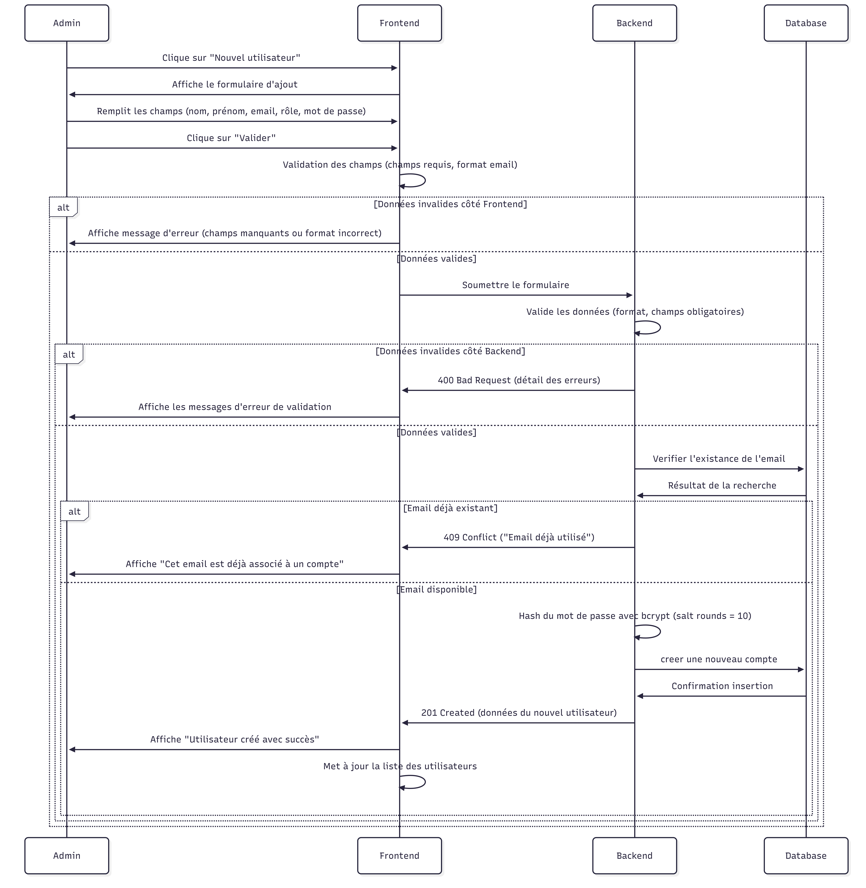
\includegraphics[scale=0.7]{project/images/ajouter-user.png}
  \caption{Diagramme de séquence <<Ajouter un utilisateur>> }
  \label{cap:Diagramme de séquence <<Ajouter un utilisateur>>}
\end{figure}
\vspace*{\fill} % espace vertical sous
\newpage
\noindent\textbf{Diagramme de séquence : Réinitialisation du mot de passe}

\noindent La Figure \ref{cap:Diagramme de séquence <<Réinitialisation du mot de passe>>} présente le diagramme de séquence relatif à la réinitialisation du mot de passe d'un utilisateur, initié par l'administrateur.
\begin{figure}[H]
  \centering
    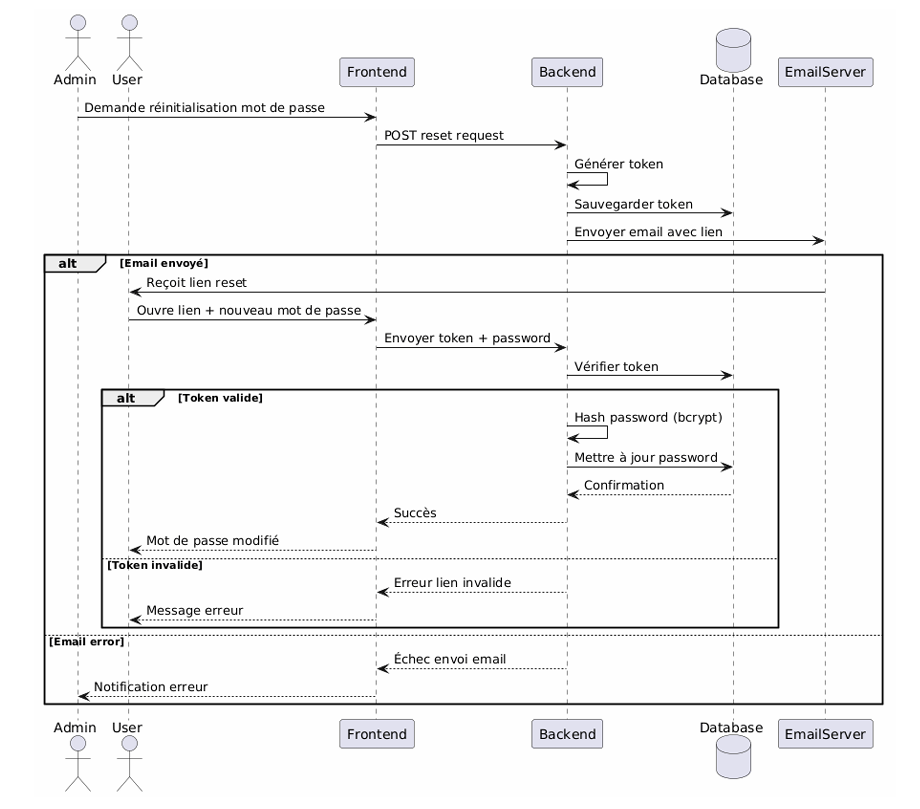
\includegraphics[scale=0.7]{project/images/admin-réinitialise.png}
  \caption{Diagramme de séquence <<Réinitialisation du mot de passe>> }
  \label{cap:Diagramme de séquence <<Réinitialisation du mot de passe>>}
\end{figure}
\vspace*{\fill} 

\newpage

\noindent \textbf{Diagramme de séquence : Gestion des demandes des apprenants}


\noindent Le diagramme de séquence de la Figure \ref{cap:Diagramme de séquence <<Gestion des demandes des apprenants>>} décrit le flux de traitement des demandes d'inscription des apprenants par l'administrateur, en détaillant les deux chemins possibles: l'acceptation, qui declanche l'envoi d'une notification par email, et le refus, qui archive la demande et notifie l'apprenant.
\begin{figure}[H]
  \centering
    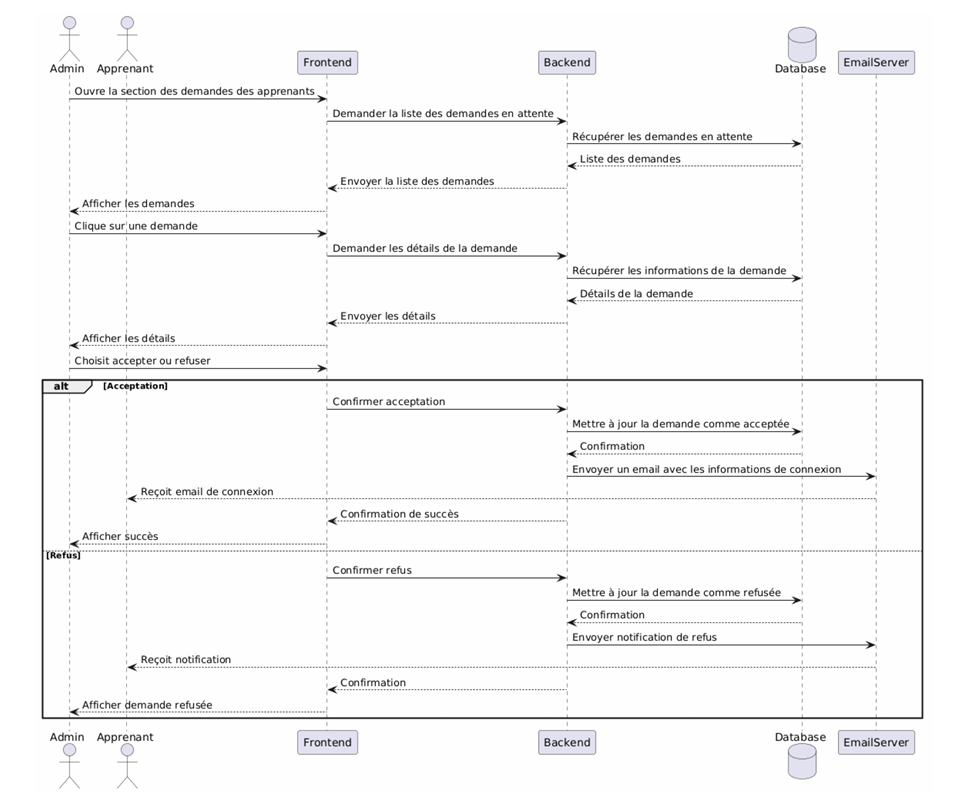
\includegraphics[scale=0.7]{project/images/accept-rejectsequence.png}
  \caption{Diagramme de séquence <<Gestion des demandes des apprenants>> }
  \label{cap:Diagramme de séquence <<Gestion des demandes des apprenants>>}
\end{figure}

\subsection{Réalisation}
Cette section présente les interfaces de gestion des utilisateurs, en mettant l’accent sur les différentes fonctionnalités implémentées et l’expérience utilisateur offerte par ces interfaces.

\vspace{0.3cm}
\noindent \textbf{Interface de gestion des utilisateurs :} 

\noindent La figure \ref{fig:capture_userstab} présente l'interface principale affichant la liste des utilisateurs sous forme de tableau structuré, avec barre de recherche et filtres par rôle.

\begin{figure}[H]  % [H] bech t7otha houni just
    \centering
    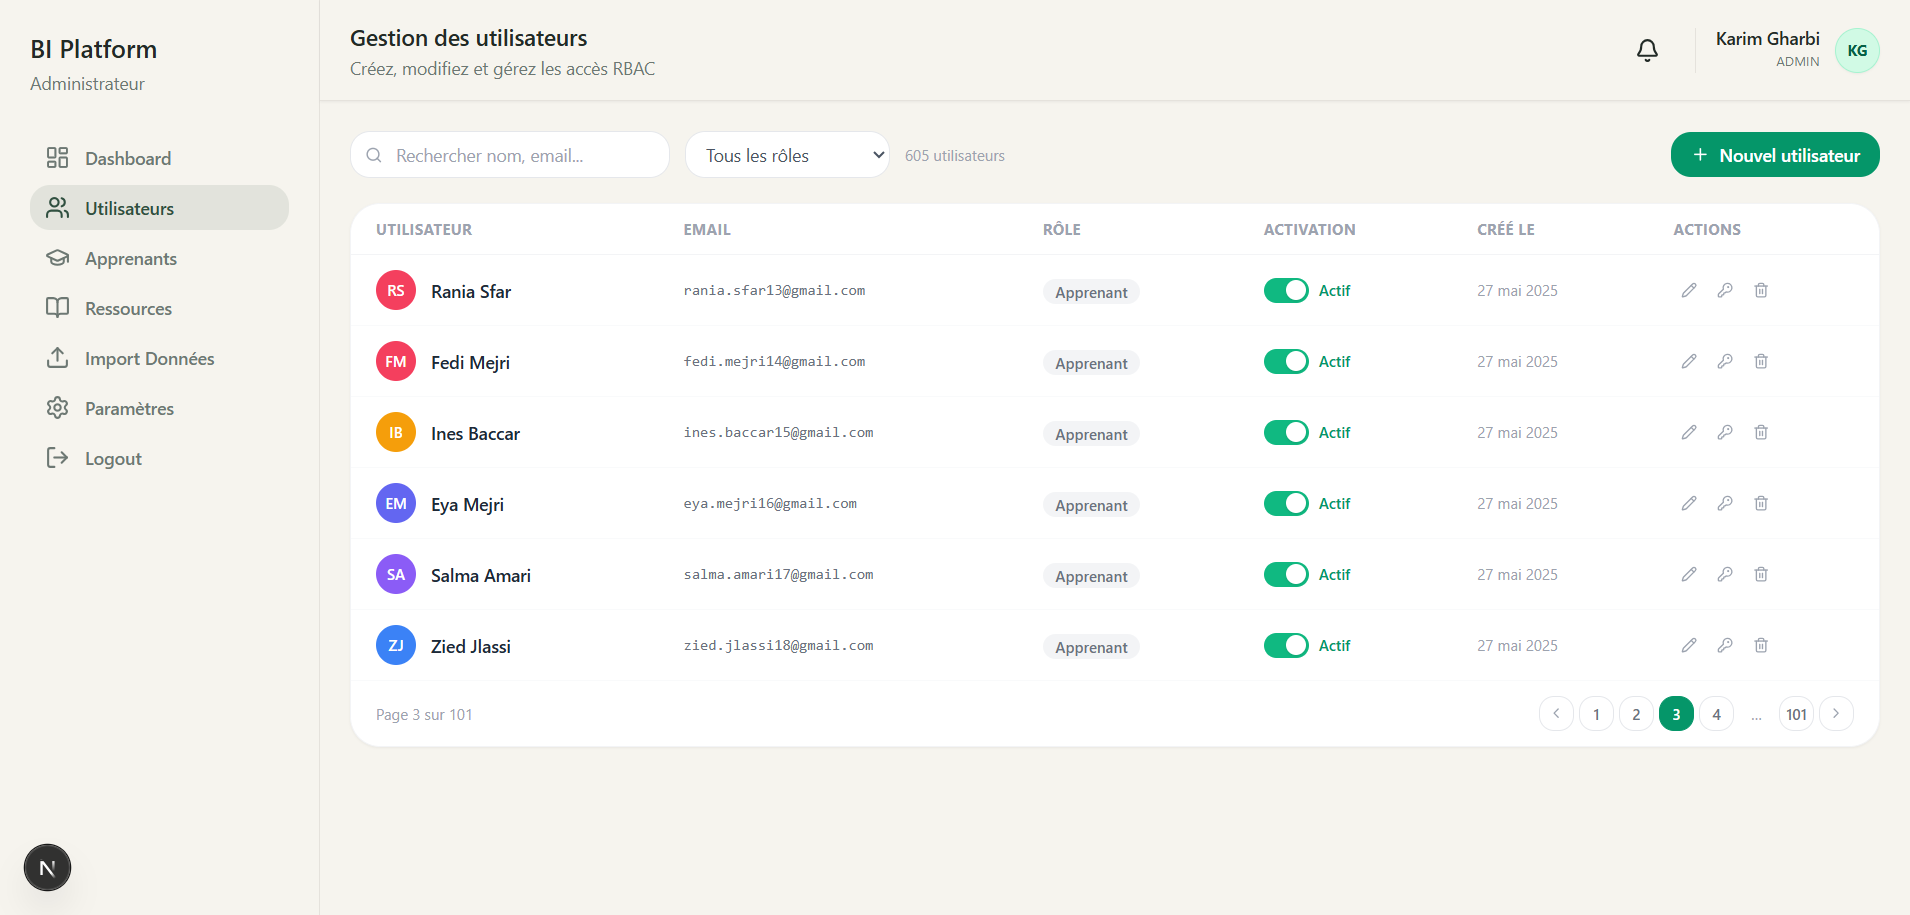
\includegraphics[width=0.8\textwidth]{project/images/localhost_3000_admin_users.png}
    \caption{Gestion des utilisateurs}
    \label{fig:capture_userstab}
\end{figure}

\noindent\textbf{Validation des comptes :} 

\noindent La figure \ref{fig:capture_learnersvalidated} illustre l'interface de traitement des demandes d'inscription, permettant à l'administrateur d'accepter ou de refuser les comptes en attente.

\begin{figure}[H]  % [H] bech t7otha houni just
    \centering
    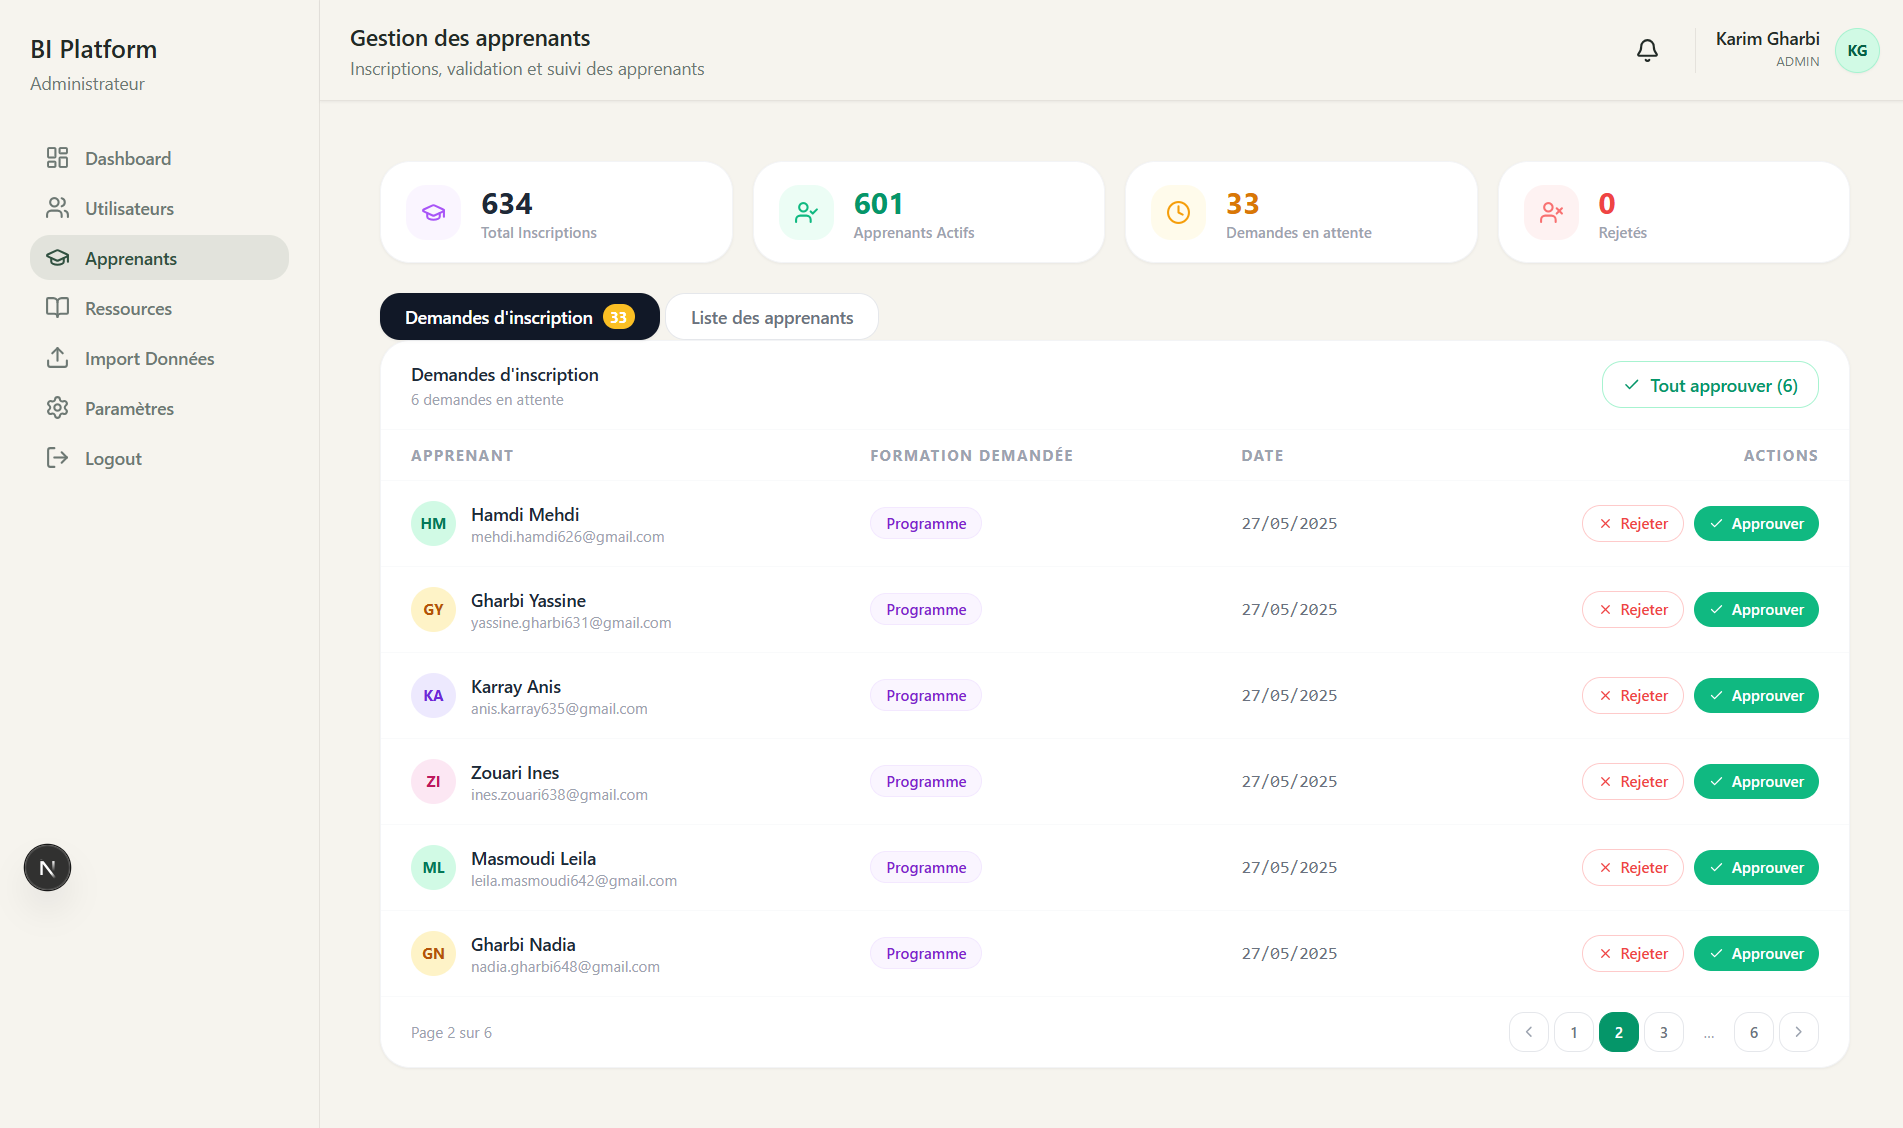
\includegraphics[width=0.9\textwidth]{project/images/localhost_3000_admin_learners.png}
    \caption{Gestion des demandes d'inscription des apprenants}
    \label{fig:capture_learnersvalidated}
\end{figure}

\noindent \textbf{Ajout d’un utilisateur :} 

\noindent La figure \ref{fig:capture_newuser} montre le modal d'ajout d'un nouvel utilisateur, comportant les champs nom, email, rôle et mot de passe.

\begin{figure}[H]  % [H] bech t7otha houni just
    \centering
    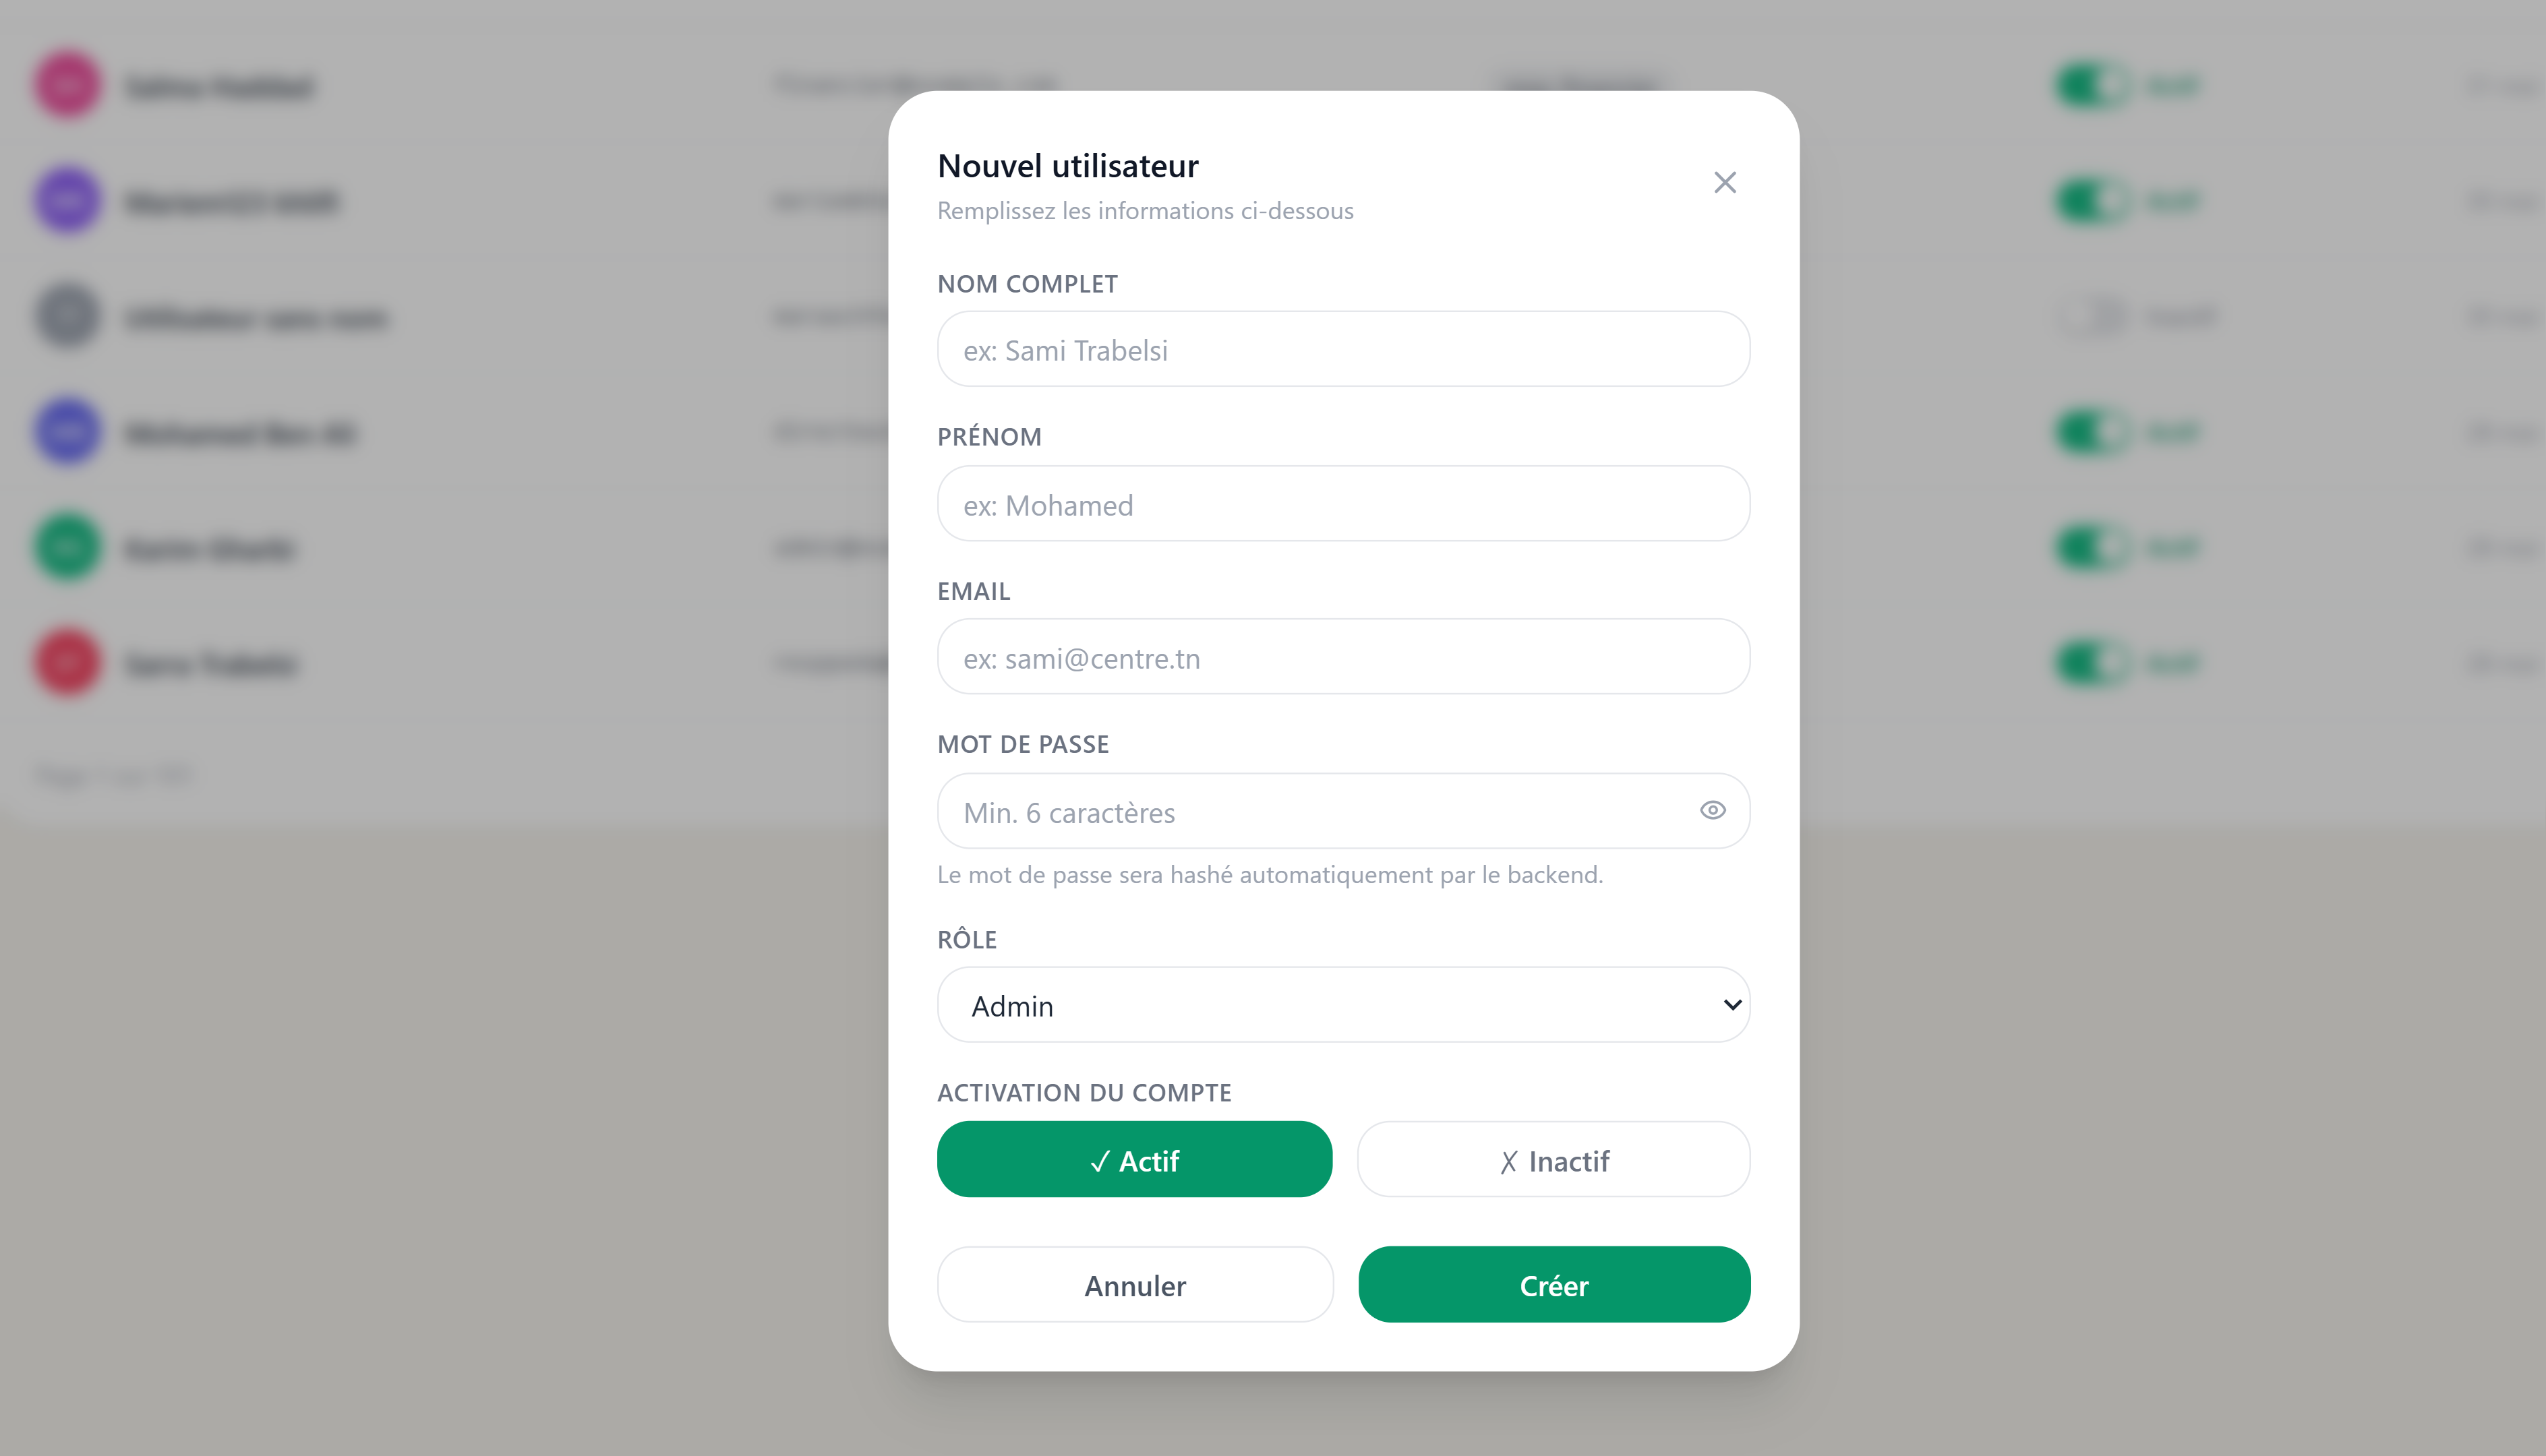
\includegraphics[width=0.8\textwidth]{project/images/newusers.png}
    \caption{Ajout d’un utilisateur}
    \label{fig:capture_newuser}
\end{figure}
\noindent \textbf{Modification des informations :} 

\noindent Les figures \ref{fig:reset-password} et \ref{fig:modifier-user} présentent respectivement la sélection d'un utilisateur et le modal de modification pré-rempli avec ses données actuelles.
\begin{figure}[H]
    \centering
    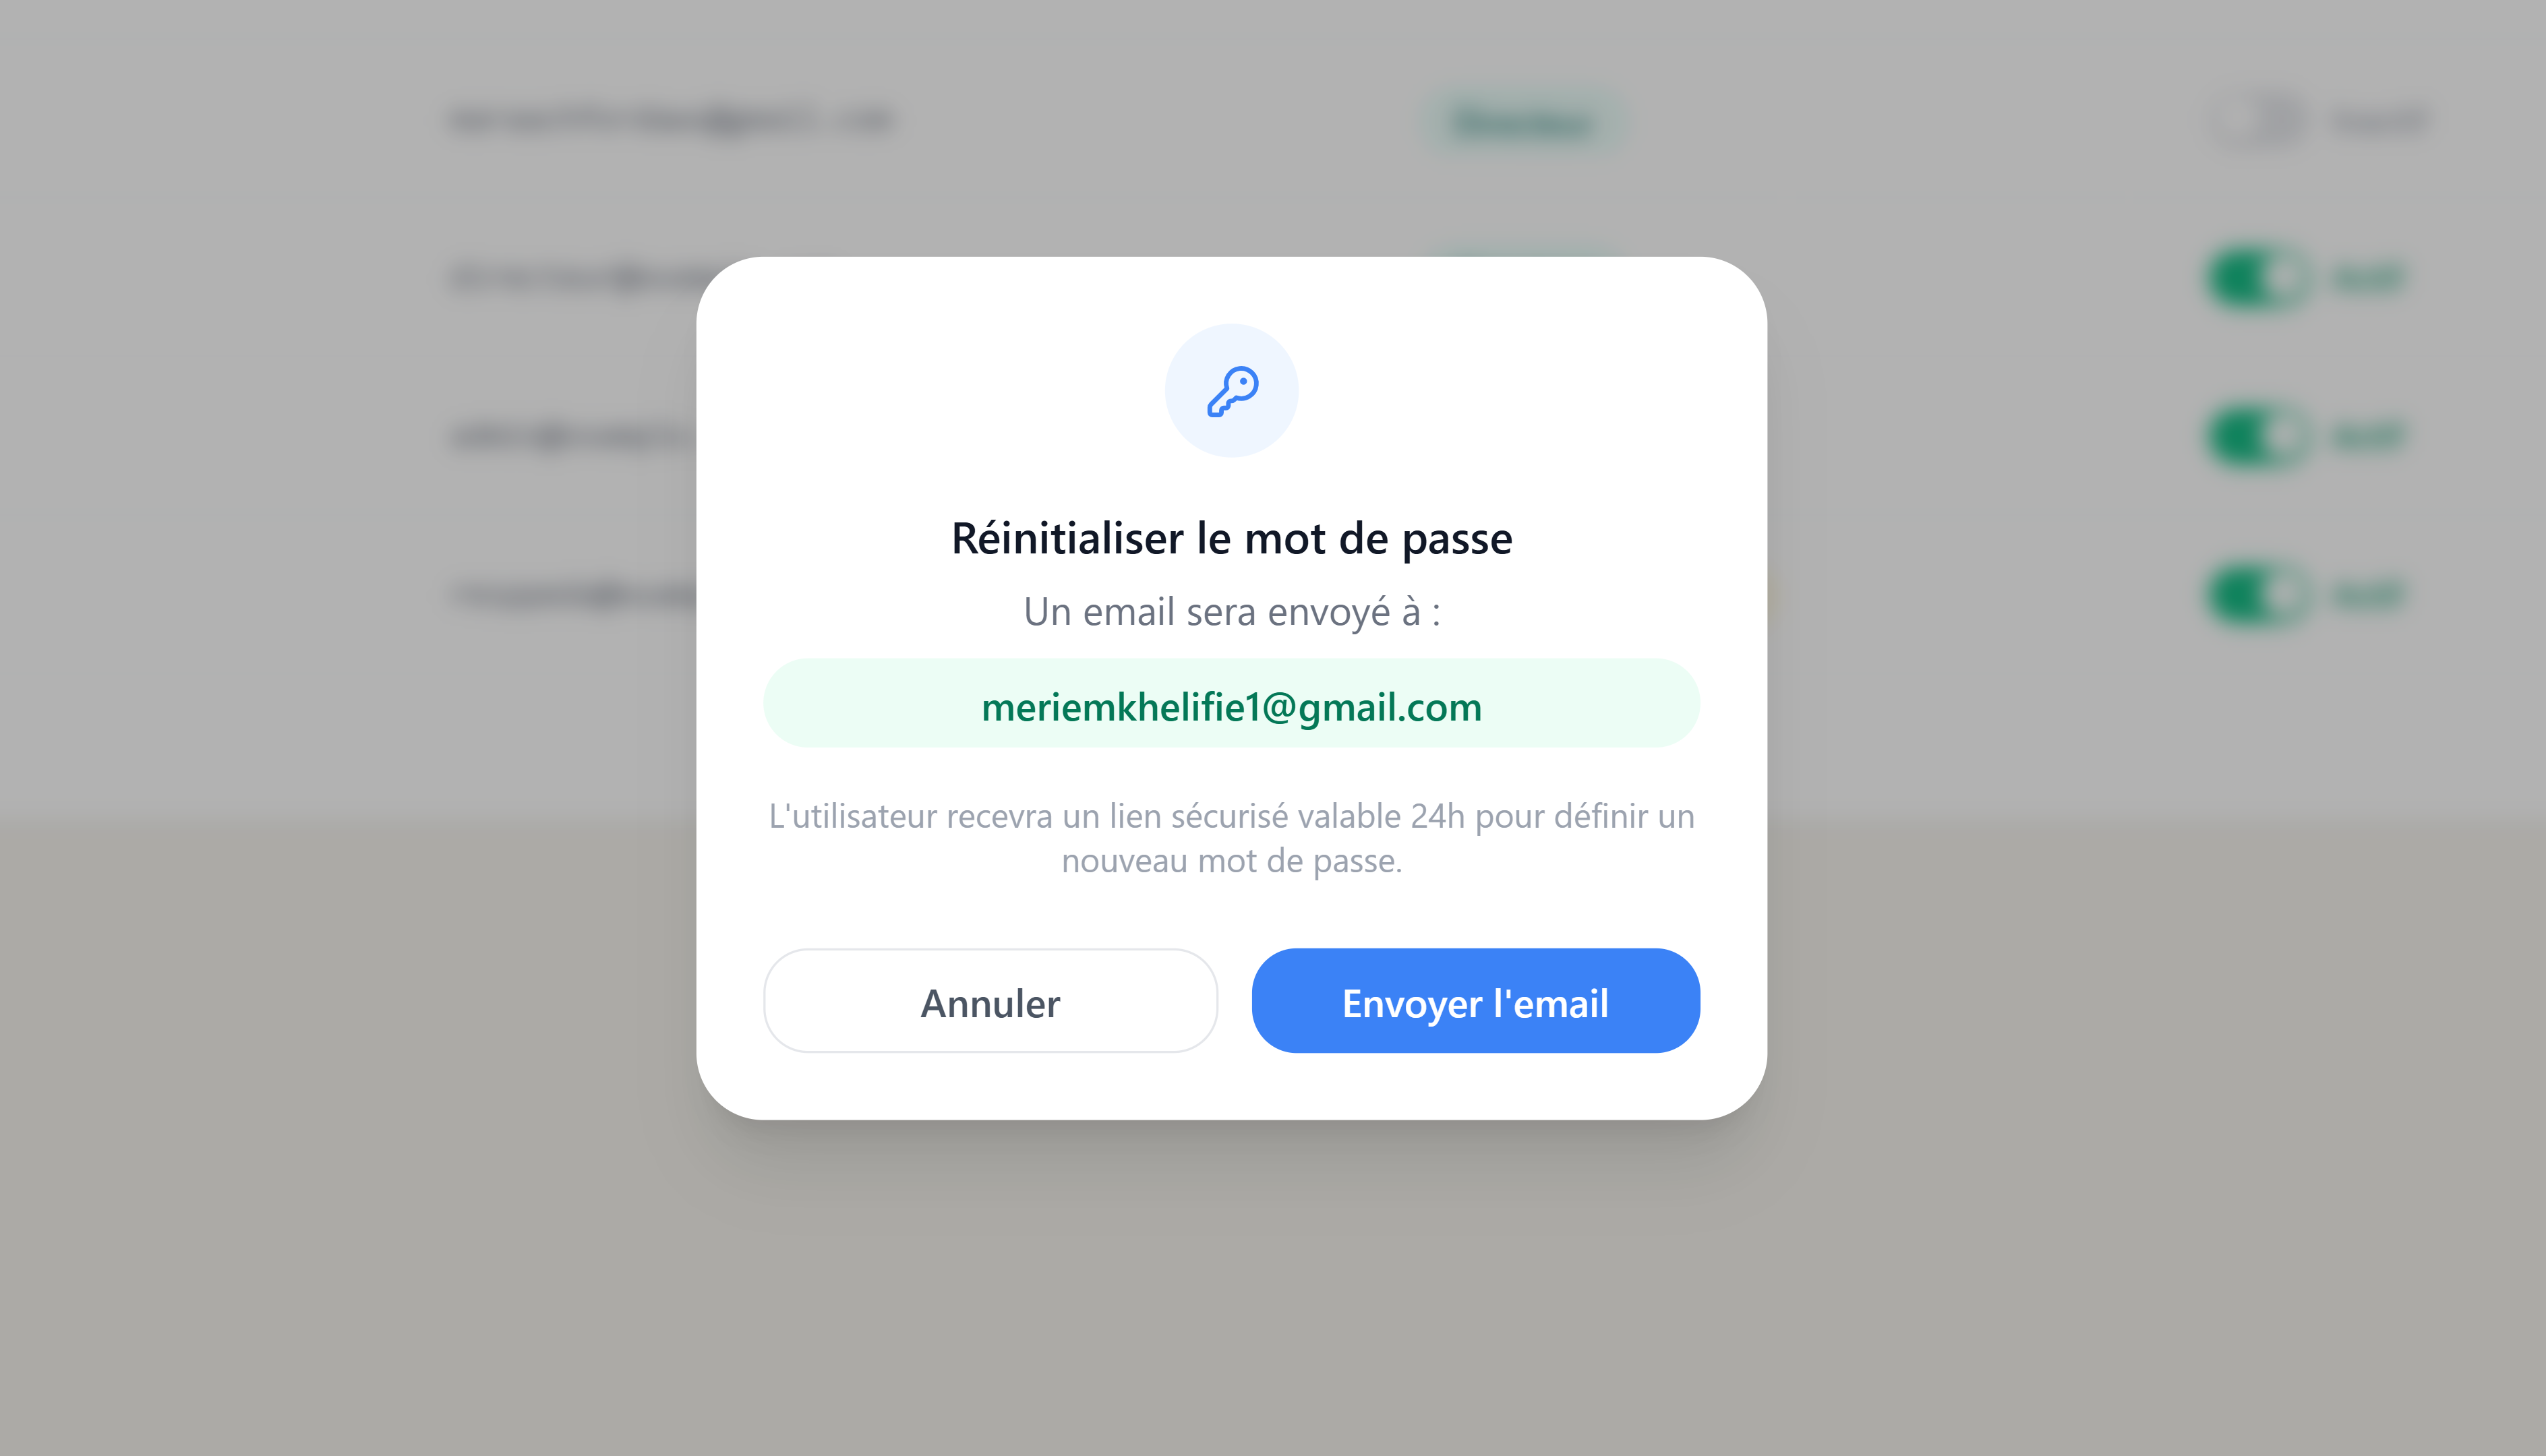
\includegraphics[width=0.6\textwidth]{project/images/resetPassword.png}
    \caption{Réinitialisation du mot de passe}
    \label{fig:reset-password}
\end{figure}

\begin{figure}[H]
    \centering
    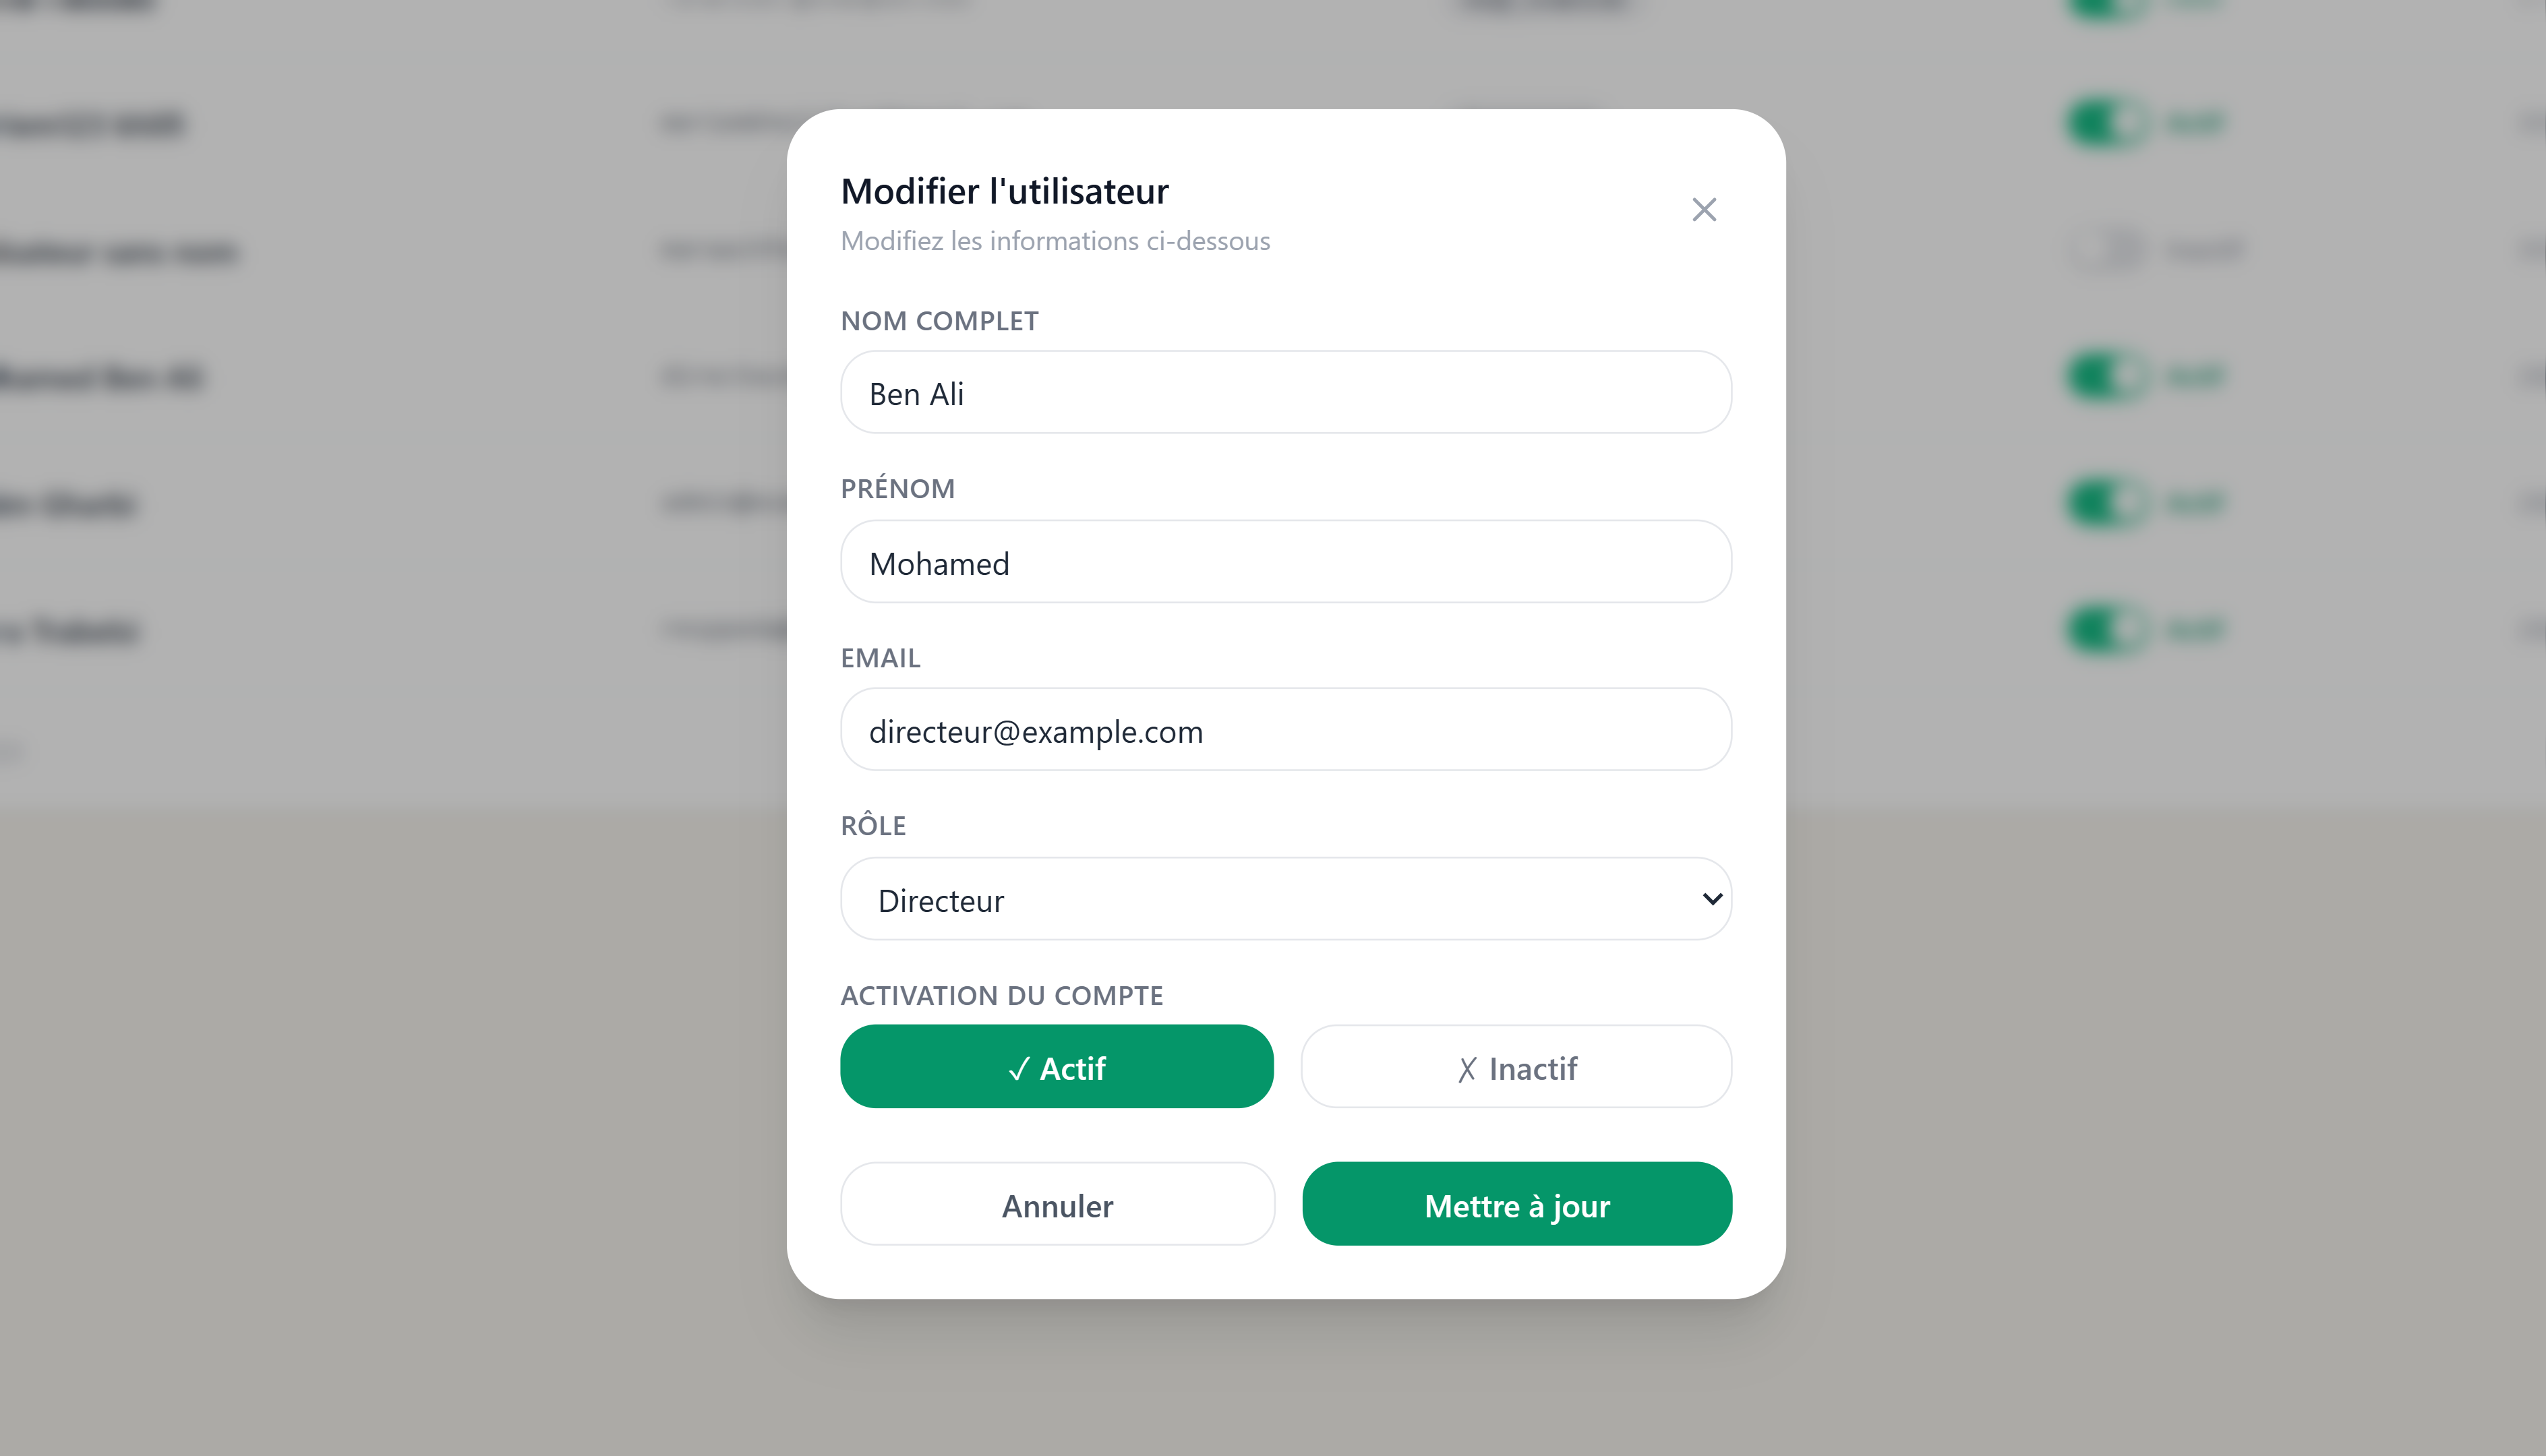
\includegraphics[width=0.6\textwidth]{project/images/ModfierUSERS.png}
    \caption{Modification d'un utilisateur}
    \label{fig:modifier-user}
\end{figure}

\textbf{Suppression d’un utilisateur :} 

\noindent La figure \ref{fig:capture_del} montre le modal de confirmation de suppression, invitant l'administrateur à confirmer ou annuler la suppression définitive du compte.

\begin{figure}[H]  % [H] bech t7otha houni just
    \centering
    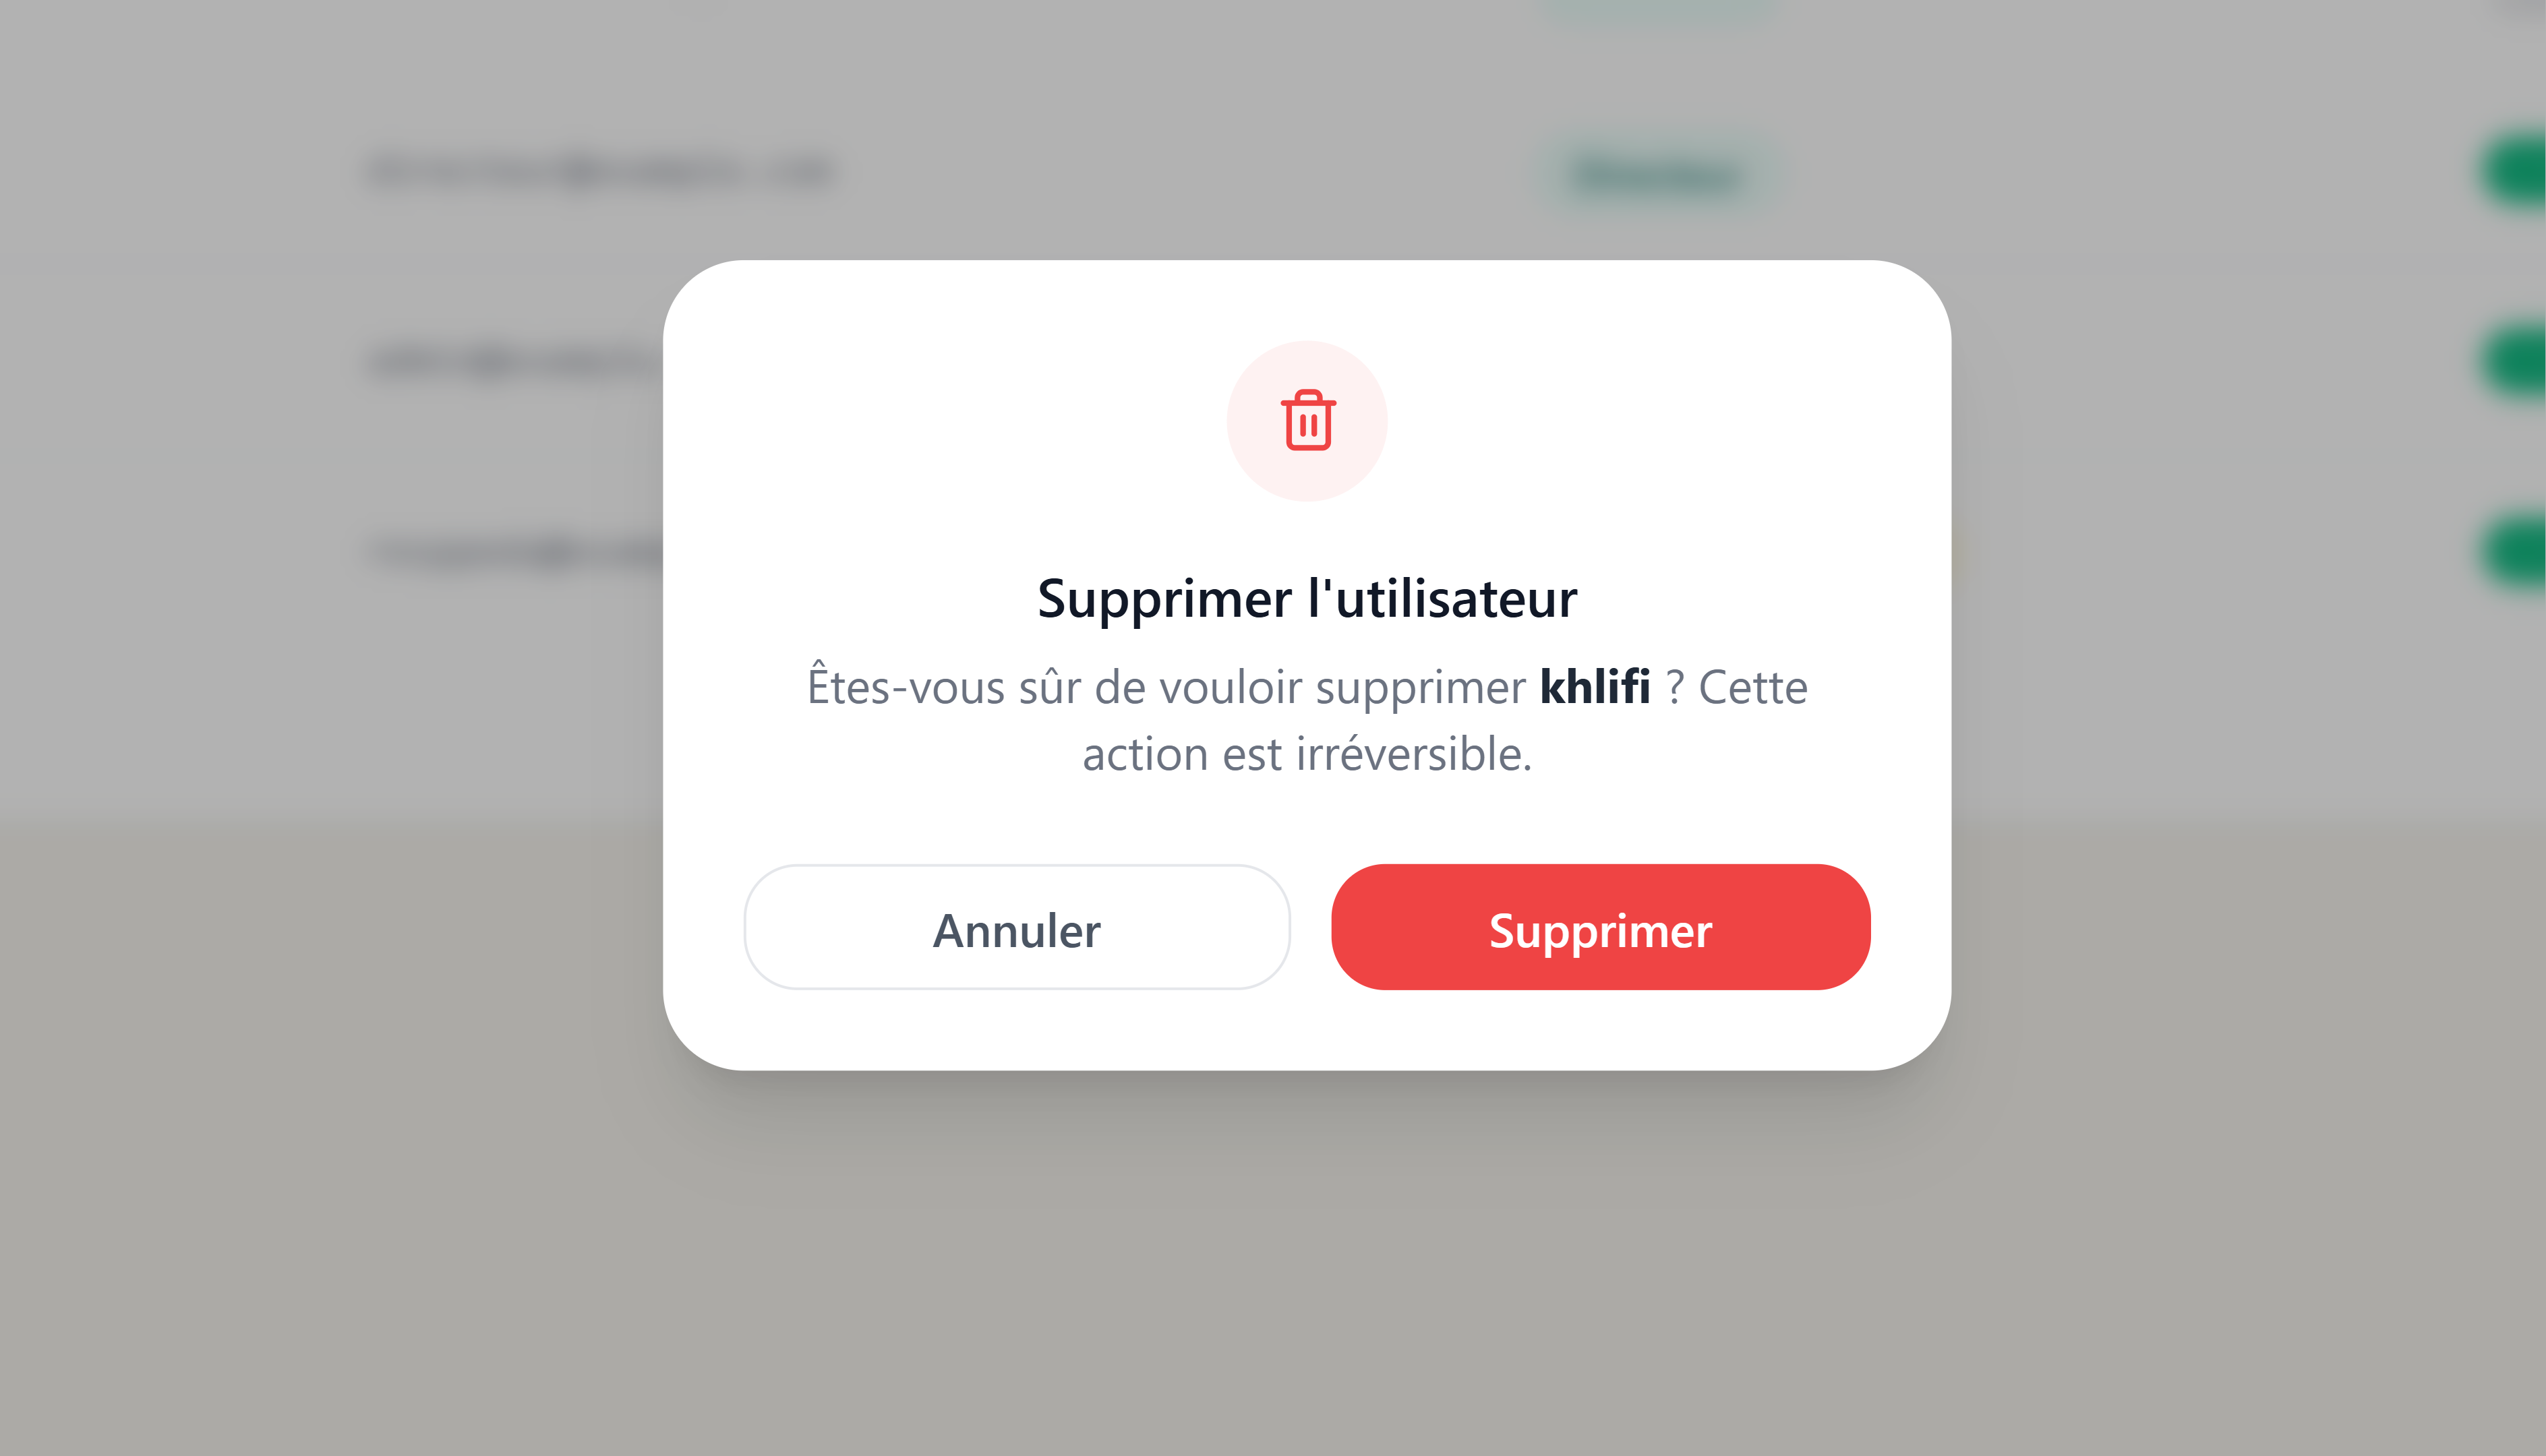
\includegraphics[width=0.8\textwidth]{project/images/deleteUsers.png}
    \caption{Suppression d'un utilisateur}
    \label{fig:capture_del}
\end{figure}

\section{Conclusion}
Ce chapitre a présenté la première release de la plateforme, organisée en deux sprints principaux. Le premier sprint a concerné la mise en place de l’authentification afin de sécuriser l’accès au système, tandis que le second a porté sur la gestion des utilisateurs et des rôles.

\noindent L’ensemble du développement a suivi une démarche structurée basée sur l’analyse, la conception et la réalisation. Cette première version constitue une base fonctionnelle importante pour la suite du projet.